\chapter{Modultest}
Ved modultests blev én funktionalitet testet isoleret. Det vil sige med så lidt påvirkning fra resten af systemet som muligt. Modultests blev udført før integrationstests, for at sikre individuel funktionalitet før sammensætning af alle komponenter. Modultests blev udført både for software-komponenter og hardware-komponenter.

\section{Software}
Til modultest af software er der gjort brug af white-box testing. Dette er gjort, da softwaren ligger tæt op ad hardwaren til kommunikationsbusserne, hvilket kræver teknisk viden om den interne struktur for både hardware og software.

\subsection{Opsummering}
\subsubsection{Wii-Nunchuck}
Dataoverførsel fra Wii-Nunchuck sker ved at PSoC0 først sender et \textit{handshake}, hvilket er en enkelt byte med værdien 0x00. Herefter kan PSoC0 aflæse Wii-Nunchuck tilstanden ved kontinuert at sende en byte med værdien \textit{??}, efterfulgt af den egentlig aflæsning. Det er altså disse to dele der skal testes på.

For flere tekniske detaljer, samt billeder af målingerne, refereres til \textbf{DOKUMENTATION \#ref}

Tabel \ref{table:modulTestNunchuckHandShake} og \ref{table:modulTestNunchuckReading} præsenterer modultest resultaterne for Wii-Nunchuck.

\begin{table}[H]
	\centering
	\begin{tabular}{ll}
		\hline
		Forventet Resultat & \begin{tabular}[c]{@{}l@{}}På I2C Bussen måles et \textit{ACKNOWLEDGE} fra Wii-Nunchuck \\ slaven når den får tilsendt et handshake fra PSoC0. Det skal \\ desuden kunne ses at en byte med værdien 0x00 modtages \\ af Wii-Nunchuck. \end{tabular} \\
		\rowcolor[HTML]{CBCEFB} 
		Egentlig Resultat  & \begin{tabular}[c]{@{}l@{}}Et \textit{ACKNOWLEDGE} blev målt som forventet, \\ og handshake byten med værdi 0x00 blev modtaget korrekt. \end{tabular}                                       \\ \hline
	\end{tabular}
	\caption{Modultest af Wii-Nunchuck Handshake}
	\label{table:modulTestNunchuckHandShake}
\end{table}

\begin{table}[H]
	\centering
	\begin{tabular}{ll}
		\hline
		Forventet Resultat & \begin{tabular}[c]{@{}l@{}}På I2C bussen måles en aflæsning af bytes fra Wii-Nunchuck\\ slaven.\end{tabular}                \\
		\rowcolor[HTML]{CBCEFB} 
		Egentlig Resultat  & \begin{tabular}[c]{@{}l@{}}På målingen af I2C bussen ses det at bytes bliver aflæst fra\\ Wii-Nunchuck slaven.\end{tabular} \\ \hline
	\end{tabular}
	\caption{Modultest af Wii-Nunchuck Data Aflæsning}
	\label{table:modulTestNunchuckReading}
\end{table}

Det kan på tabel \ref{table:modulTestNunchuckHandShake} og \ref{table:modulTestNunchuckReading} ses at de egentlige resultaterne stemte overens med de forventede.

\subsubsection{I2C Kommunikationsprotokol}
I2C Kommunikationsprotokollen beskrevet i afsnit \ref{afsnit:I2CProtokol} blev modultestet ved to tests. Den første test er til for at verificere at kommandotyper bliver overført på I2C bussen i korrekt format. Den anden test er til for at verificere at modtaget I2C data fortolkes korrekt af software på PSoC0.

\begin{table}[H]
	\centering
	\begin{tabular}{ll}
		\hline
		Forventet Resultat & \begin{tabular}[c]{@{}l@{}}På I2C Bussen måles kommandotypen NunchuckData \\i korrekt format.\end{tabular} \\
		\rowcolor[HTML]{CBCEFB} 
		Egentlig Resultat  & \begin{tabular}[c]{@{}l@{}}Målingen af I2C bussen viste kommandotypen \\ NunchuckData i korrekt format.  \end{tabular}                                       \\ \hline
	\end{tabular}
	\caption{Modultest af kommandotype på I2C Bussen}
	\label{table:modulTestCommandFormat}
\end{table}

\begin{table}[H]
	\centering
	\begin{tabular}{ll}
		\hline
		Forventet Resultat & \begin{tabular}[c]{@{}l@{}} \end{tabular} \\
		\rowcolor[HTML]{CBCEFB} 
		Egentlig Resultat  & \begin{tabular}[c]{@{}l@{}}  \end{tabular}                                       \\ \hline
	\end{tabular}
	\caption{Modultest af kommandofortolkningssoftware}
	\label{table:modulTestI2CData}
\end{table}

\subsubsection{SPI Kommunikationsprotokol}

\subsubsection{Rotationsdetektor}
\begin{table}[H]
	\centering
	\begin{tabular}{|l|c|c|}
		\hline
		\textbf{Indgangssignal} & \textbf{Forventet PWM} & \textbf{Målt PWM} \\ \hline
		0V                      & Ja                     & Ja                \\ \hline
		1400mV                  & Ja                     & Ja                \\ \hline
		1500mV                  & Ja                     & Ja                \\ \hline
		1600mV                  & Nej                    & Ja                \\ \hline
		2,2V                    & Nej                    & Ja                \\ \hline
		2,3V                    & Nej                    & Nej               \\ \hline
		5V                      & Nej                    & Nej               \\ \hline
	\end{tabular}
	\caption{Modultest af ADC}
	\label{my-label}
\end{table}

\subsection{Modultest af Wii-Nunchuck}
På PSoC0 er der software til aflæsning af Wii-Nunchuck input data. Følgende afsnit beskriver test af dette software.

Aflæsning af Wii-Nunchuck sker i to skridt, som begge verificeres ved modul test. Først skal der sendes et \textit{Handshake} fra PSoC0 til Wii-Nunchuck for at initialisere data udveksling, og herefter sker data udveksling hver gang PSoC0 sender en anmodning om det. Disse to skridt modultestes her.

\textbf{Test af Wii-Nunchuck Handshake}

\textbf{Test af data udveksling mellem PSoC0 og Wii-Nunchuck} 

PSoC0 blev programmeret til kontinuert aflæsning af Wii-Nunchuck. For at verificere data udveksling mellem PSoC0 og Wii-Nunchuck blev I2C bussen målt ved brug af Logic Analyzer fra Analog Discovery.

Data udveksling sker i to skridt. Først sender PSoC0 en byte med værdien 0 (0x00 i hexadecimal). Herefter sker den faktiske aflæsning, PSoC0 aflæser Wii-Nunchuck. Begge skridt testes her.

\textbf{Afsendelse af 0x00 byte}

Den første forventede I2C besked er en \textit{0x00} byte fra PSoC0 for at starte en ny aflæsning. På figur \ref{fig:NunchuckWriteValues} ses aflæsningen af I2C bussen på tidspunktet hvor anmodningen til Wii-Nunchuck bliver udført. Dette er en tidslinje læst fra ventre til højre.

\begin{figure}[H]
	\centering
	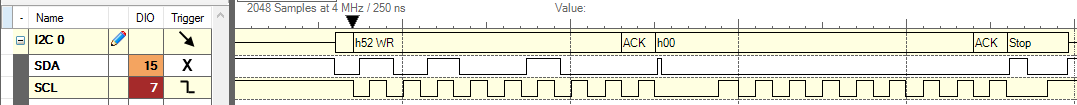
\includegraphics[width=\textwidth]{Test/images/writerequest}
	\caption{}
	\label{fig:NunchuckWriteValues}
\end{figure}

Det kan på figur \ref{fig:NunchuckWriteValues} ses at den første besked der måles er af typen "WR" (Write) til addressen 0x52 (Wii-Nunchuck I2C Slave Addressen). Hertil kommer et tilhørende \textit{ACK} (Acknowledge) fra Wii-Nunchuck. Til sidst sendes dataen Ox00 efterfulgt af at ACK fra Wii-Nunchuck. Til sidst afsluttes I2C transaktionen ved "Stop".

Det kan altså konkluderes at målingen er i overensstemmelse med forventningen om at en 0x00 byte skal sendes til Wii-Nunchuck for opstart af dataudveksling.

\textbf{Aflæsning af Wii-Nunchuck}

Efter vellykket afsendelse af 0x00 byten sker den egentlige aflæsning af Wii-Nunchuk input dataen.

Her forventes en række beskeder indeholdende 

På figur \ref{fig:NunchuckReadValues} ses I2C beskederne der bliver udvekslet mellem PSoC0 og Wii-Nunchuck efter vellykket Wii-Nunchuck Handshake. 

\begin{figure}[H]
	\centering
	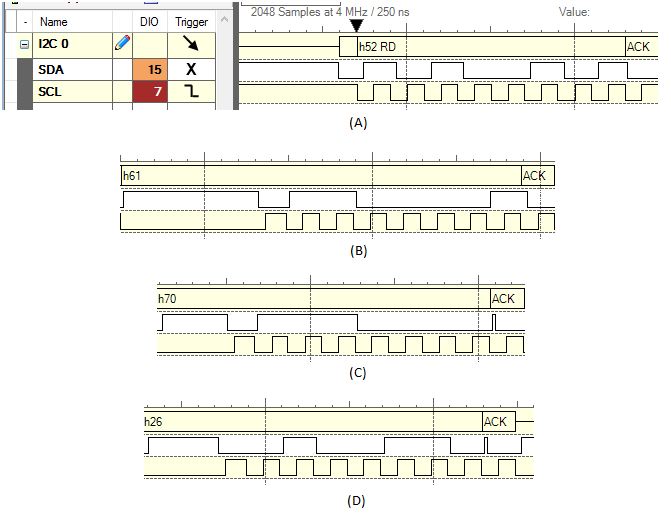
\includegraphics[width=\textwidth]{Test/images/readvaluesEdited.png}
	\caption{Tidslinje af aflæste I2C beskeder af PSoC0 fra Wii-Nunchuck}
	\label{fig:NunchuckReadValues}
\end{figure}

\subsection{SPI Protokol}
Devkittet kommunikerer over en SPI bus. Kommunikationen følger SPI kommunikations protokollen, som er beskrevet i afsnit \ref{afsnit:spiprotokol}. Dette afsnit beskriver test af denne protokol.

\subsubsection{SPI Bus Test}
Test af SPI bussen udføres i to dele. Første del af testen udføres ved at sende kommandotypen for start af SPI test i terminalen, og derefter verificere den sendte data vha. Analog Discovery. Den anden del af testen, er at aflæse returbeskeden på bussen med Analog Discovery. Målet med denne test, er at læse kommandotypen "SPI\_OK", der indikerer en successful aflæsning af SPI-slaven.  På figur \ref{figure:SpiTestSetup} ses test opsætningen. Devkit8000, PSoC0s SPI-bus og Analog Discovery  er forbundet til hinanden igennem fumlebrættet. PSoC0 og PSoC1's I2C-forbindelser forbindes til nunchucken igennem fumlebrættet, adskilt fra SPI-forbindelserne.


\begin{figure}[H]
	\centering
	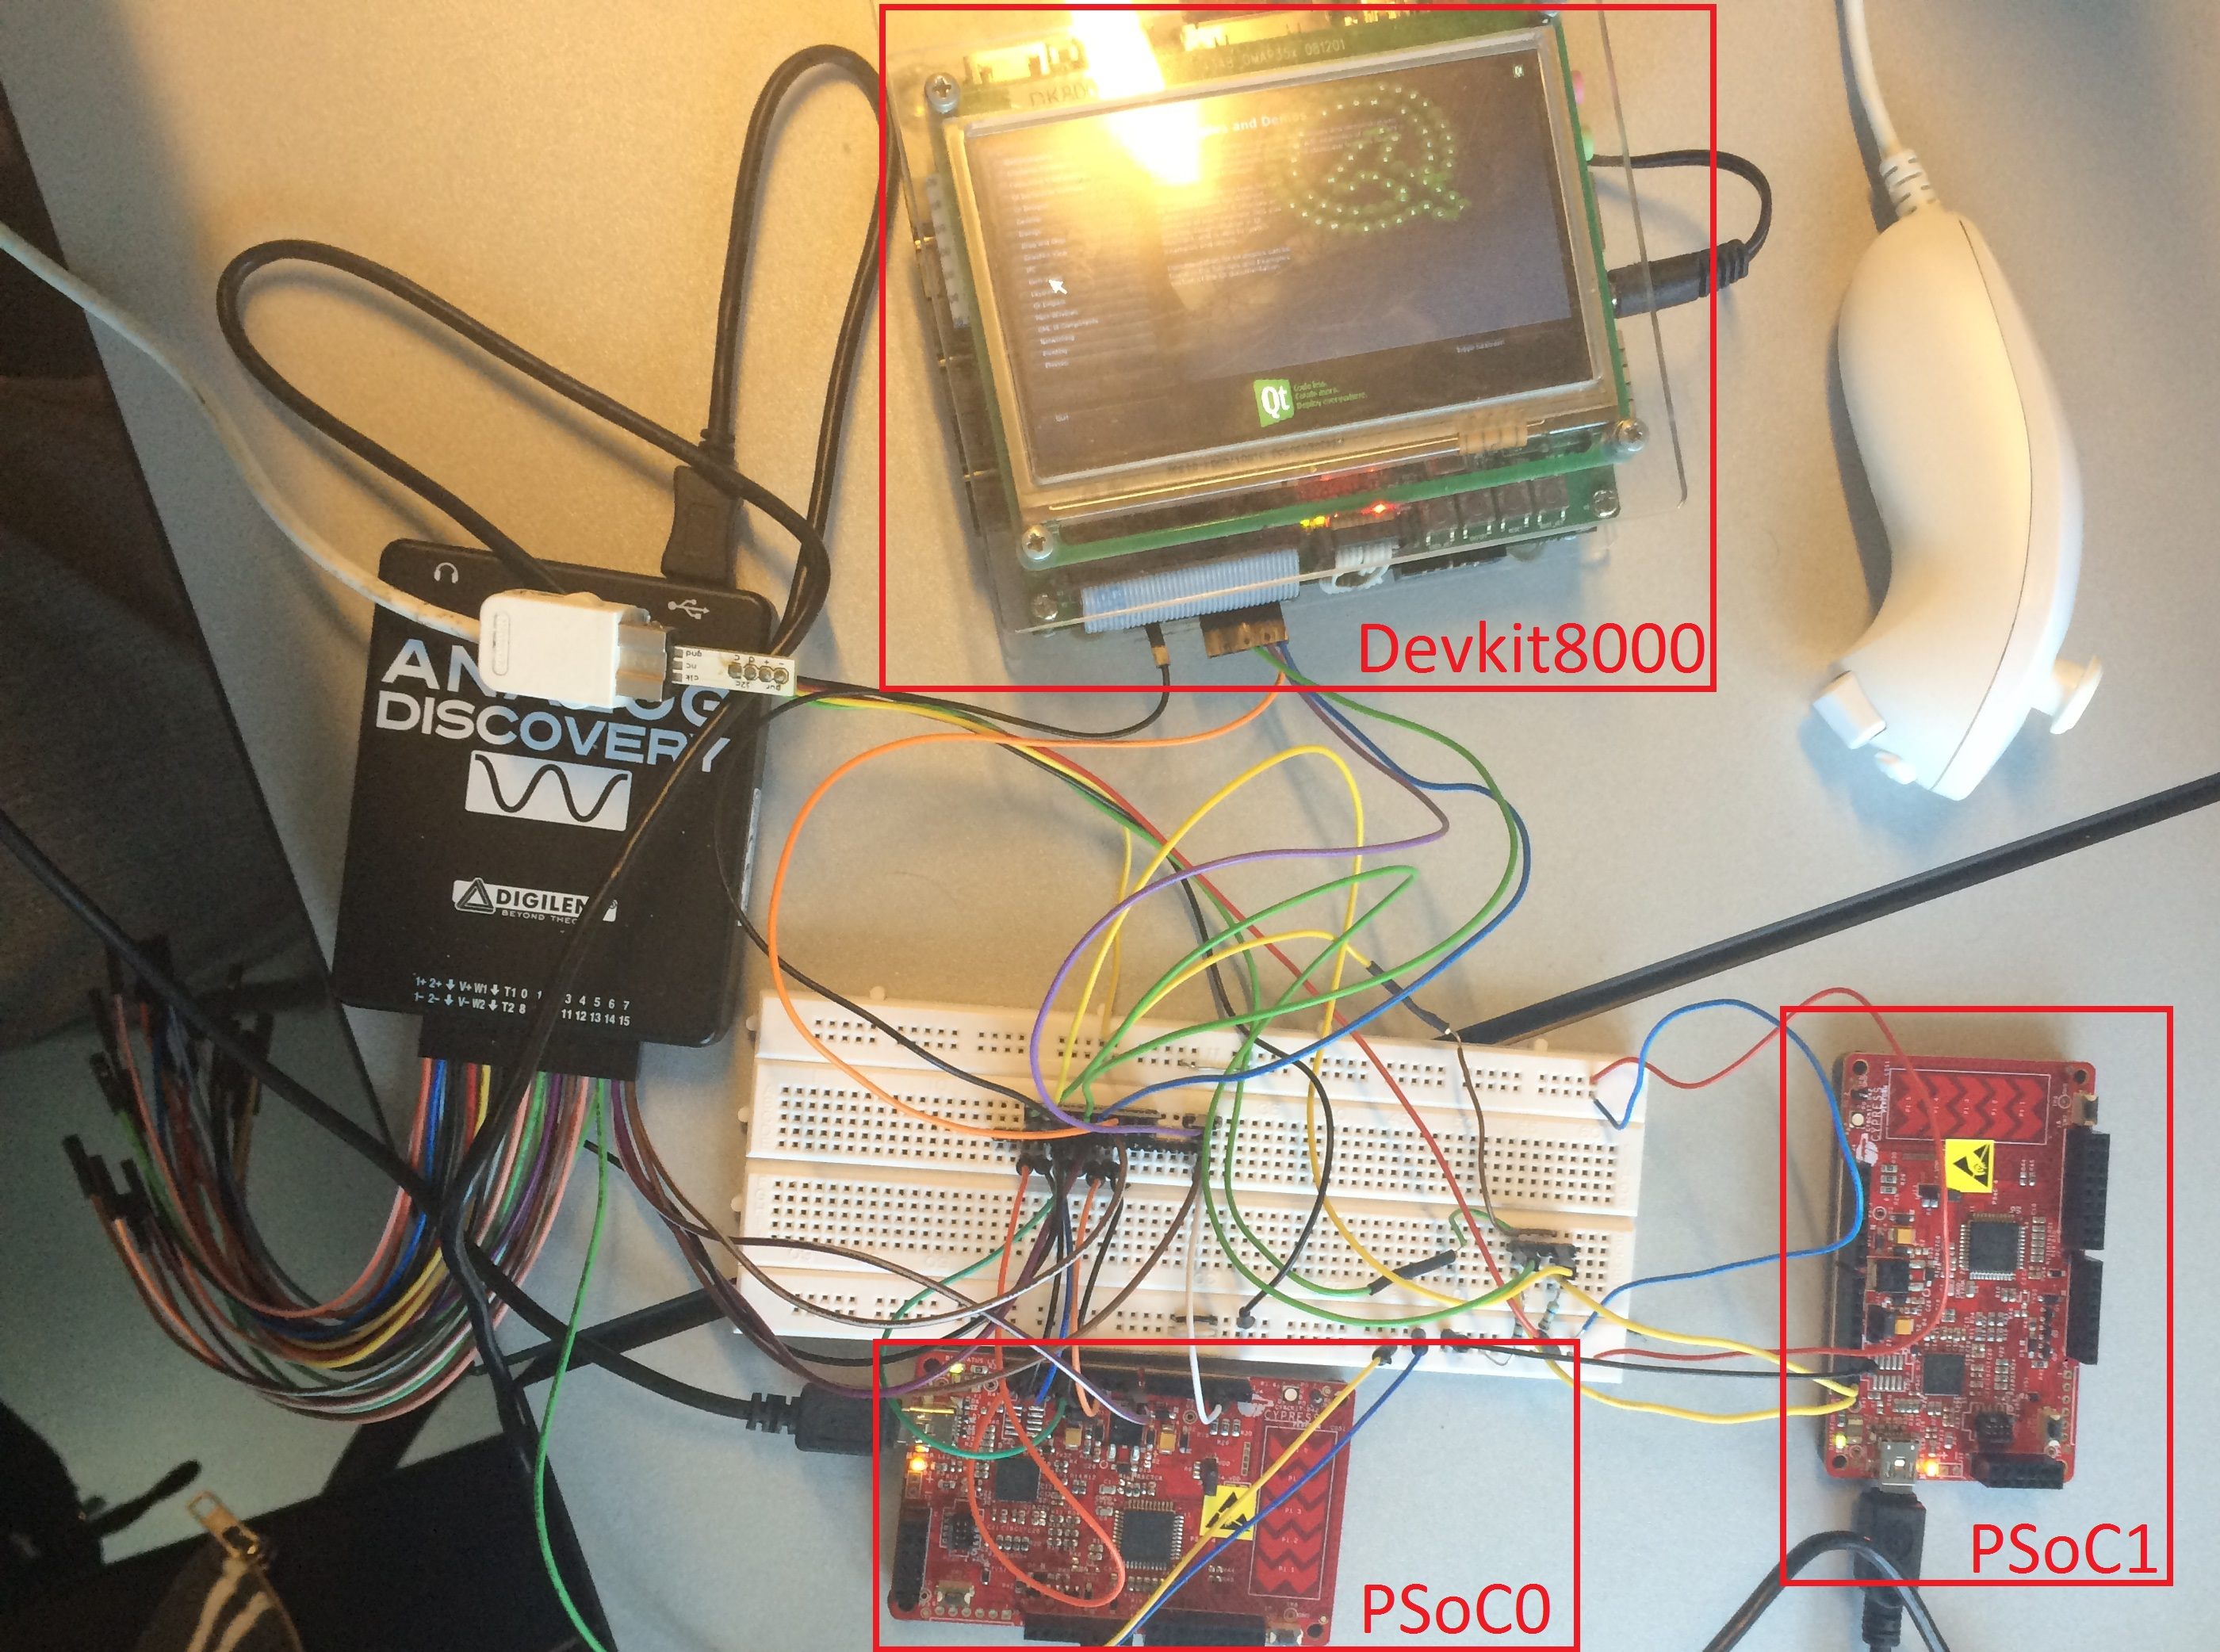
\includegraphics[width=\textwidth]{Test/images/SPItest/SpiTestSetup}
	\caption{Opsætning for SPI-test}
	\label{figure:SpiTestSetup}
\end{figure}


I testen afsendes SPI test kommandotypen, som har værdien 0xF1 jf. tabel \ref{tabel:spiKommandoType}. For at verificere, at kommandotypen er sendt ud på SPI-bussen korrekt, blev Analog Discovery's 'Logic Analyzer' brugt til at aflæse SPI-bussen. Det var forventet at 0xF1 blev aflæst på bussen. Det afmålte resultat stemte overens med det forventede. Målingen ses på figur \ref{fig:SPItestkommandotype}. 

\begin{figure}[H]
	\centering
	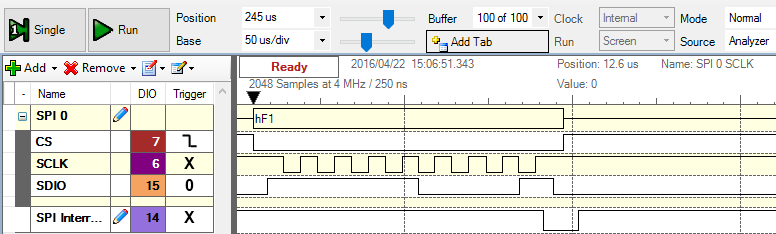
\includegraphics[width=\textwidth]{Test/images/SPItest/SPItestkommandotype}
	\caption{Måling af kommandotype for start SPI test}
	\label{fig:SPItestkommandotype}
\end{figure}

Hvis SPI-kommunikationen fungerer korrekt, er det forventet at der aflæses 0xD1 på SPI-bussen, da dette betyder 'SPI\_OK' jf. tabel \ref{tabel:spiKommandoType}. Måling af returbeskeden ses på figur \ref{fig:SPItestSPIOK}.

\begin{figure}[H]
	\centering
	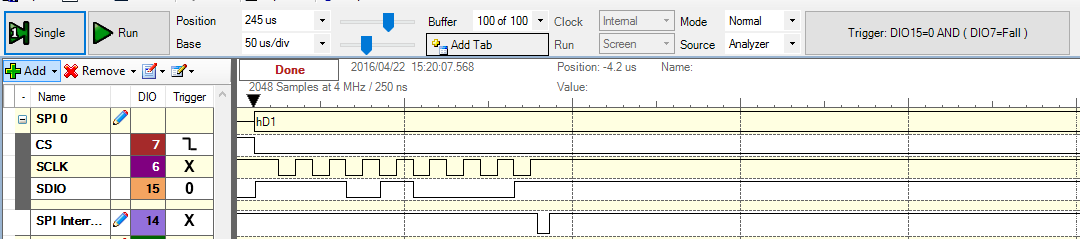
\includegraphics[width=\textwidth]{Test/images/SPItest/SPItestSPIOK1}
	\caption{Måling af returbesked for start SPI test} 
	\label{fig:SPItestSPIOK}
\end{figure}

På figur \ref{fig:SPItestSPIOK} ses at returbeskeden har den forventede værdi 0xD1, som indikerer at SPI bus testens første del er gennemført uden fejl.

Ud fra testenes resultater kan det konkluderes at implementeringen af SPI protokollen fungerer efter hensigten.



\subsection{I2C Protokol}
PSoC0 og PSoC1 kommunikerer over en I2C bus via I2C protokollen beskrevet i afsnit \ref{afsnit:I2CProtokol}. Dette afsnit beskriver test af denne protokol. Følgende test tager udgangspunkt i kommandotypen \textit{NunchuckData} beskrevet i tabel \ref{table:I2CKommandoer}).

\subsubsection{Test af NunchuckData kommandotype} 

Testen blev udført i to dele. I første del måles I2C bussen ved brug af Analog Discovery's Logic Analyzer; for at verificere at den forventede kommandotype bliver overført via bussen. Anden del verificerer at den overførte data er modtaget korrekt via PSoC Creator's debugger.

\subsubsection{NunchuckData kommandotype test del 1}

I testen afsendes, som nævnt i afsnittets indledning, kommandotypen NunchuckData. Som vist i tabel \ref{table:I2CKommandoer} har denne kommandotype ID'et 0xA2, hvor de efterfølgende 3 data bytes indeholder input dataen fra Wii-Nunchuck.

Det forventede resultat af målingen er at første byte er kommandoentypens ID, som har værdien 0x2A. Kommandoens data - de efterfølgende bytes - verificeres først i anden del, disse indgår altså ikke i følgende måling. 

Målingen ses på figur \ref{fig:NunchuckDataCommand}.

\begin{figure}[H]
	\centering
	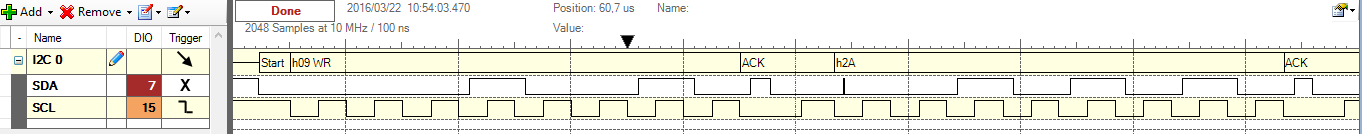
\includegraphics[width=1.2\textwidth]{Test/images/ShowsNunchuckDataCommand.png}
	\caption{Tidslinje af målt I2C kommandotype}
	\label{fig:NunchuckDataCommand}
\end{figure}

Det kan ses på figur \ref{fig:NunchuckDataCommand} at I2C overførslen starter med en I2C \textit{write}, som får et successfuldt acknowledge fra slaven PSoC1. Herefter kan det ses at den næste byte der sendes har værdien 0x2A. Denne byte er kommandoentypens ID, og er altså som forventet 0x2A.

Det kan altså verificeres at kommandoen overføres via I2C bussen. Dataens integritet er dog ikke inkluderet i denne del, og testes i del 2.

\subsubsection{NunchuckData kommandotype test del 2}
For at verificere integriteten af den data der sendes mellem PSoC0 og PSoC1, bruges PSoC Creators indbyggede debugger. Igen er det kommandotypen NunchuckData der sendes mellem de to enheder, hvor de medfølgende data bytes fortolkes.

Testen gennemføres ved at fortolke den modtagne data tre gange, hvor nunchucken er i forskellige tilstande (hvilken retning det analoge stik er trykket) i hver test. Værdierne sammenlignes de forventede standardværdier som ses i tabellen på side 3 i \cite[I2C Interface with Wii Nunchuck]{nunchuck}. Da testene kun er fokuserede på, hvilken retning den analoge stick er presset, er det altså kun receivedDataBuffer[1] (den analoge stick x-akse) og receivedDataBuffer[2] (den analoge pinds y-akse) der er relevante for testen. Når den analoge stick er presset til venstre, forventes det ifølge tabel \ref{tabel:WiiNunchuckStickPositioner} at receivedDataBuffer[1] er lig 0x1E og receivedDataBuffer[2] er 0x7B. Når den analoge stick er presset op, forventes det at receivedDataBuffer[1] er 0x7E og receivedDataBuffer[2] er 0xDF. Når der ikke er noget input på Nunchucken forventes det at receivedDataBuffer[1] er 0x7E og receivedDataBuffer[2] er 0x7B. Målingerne for testene kan ses på figur \ref{fig:I2CProtocolReadNoInput}, \ref{fig:I2CProtocolReadLeftAnalog} og \ref{fig:I2CProtocolReadUpAnalog}.

\begin{figure}[H]
	\centering
	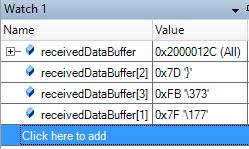
\includegraphics[width=.5\textwidth]{Test/images/I2CProtocolReadNoInput.png}
	\caption{Afmåling af modtager-buffer på PSoC1 efter at have modtaget "NunchuckData" kommando typen. Intet input på Nunchuck'en}
	\label{fig:I2CProtocolReadNoInput}
\end{figure}

\begin{figure}[H]
	\centering
	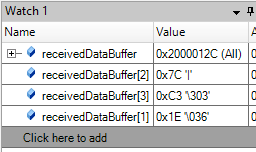
\includegraphics[width=.5\textwidth]{Test/images/I2CProtocolReadLeftAnalog.png}
	\caption{Afmåling af modtager-buffer på PSoC1 efter at have modtaget "NunchuckData" kommando typen. Den analoge stick er presset til venstre på Nunchuck'en}
	\label{fig:I2CProtocolReadLeftAnalog}
\end{figure}

\begin{figure}[H]
	\centering
	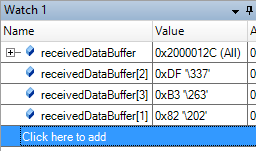
\includegraphics[width=.5\textwidth]{Test/images/I2CProtocolReadUpAnalog.png}
	\caption{Afmåling af modtager-buffer på PSoC1 efter at have modtaget "NunchuckData" kommando typen. Den analoge stick er presset frem på Nunchuck'en}
	\label{fig:I2CProtocolReadUpAnalog}
\end{figure}

På figur \ref{fig:I2CProtocolReadLeftAnalog} ses afmålingen af modtager-bufferen når Nunchuckens analoge stick er presset helt til venstre. ReceivedDataBuffer[1] blev aflæst til 0x1E og receivedDataBuffer[2] blev aflæst til 0x7C. ReceivedDataBuffer[1] stemmer overens med forventningerne. ReceivedDataBuffer[2] har en lille afvigelse (oversat til decimaltal blev der målt 124, hvor der forventes 123). Denne afvigelse kan skyldes, at det analoge stick ikke blev presset direkte til venstre, men at den også er blevet presset en smule frem under målingen.

På figur \ref{fig:I2CProtocolReadUpAnalog} ses afmålingen af modtager-bufferen når Nunchuckens analoge stick er presset frem. ReceivedDataBuffer[1] blev aflæst til 0x82, hvor det var forventet 0x7E. Dette er en afvigelse fra de forventede resultater med 4, og kan skyldes at det analoge stick ikke var helt centreret idét den blev presset frem under målingen. ReceivedDataBuffer[2] blev aflæst til 0xDF, hvilket stemmer overens med de forventede målinger.

På figur \ref{fig:I2CProtocolReadNoInput} ses afmålingen af modtager-bufferen når der ikke er noget brugerinput på nunchuckens analoge stick. ReceivedDataBuffer[1] blev aflæst til 0x7F, hvor det forventede resultat var 0x7E. Denne afvigelse kan skyldes at det analoge stick ikke stod helt i midten under målingen (Det analoge stick er lidt "løs" og kan defor godt finde hvile i en position der ikke er fuldt centreret). ReceivedDataBuffer[2] blev aflæst til 0x7D, hvor det forventede resultat var 0x7B. Igen kan denne afvigelse skyldes at det analoge stick ikke var i centrum under målingen.

Ud fra testen kan det konkluderes at implementeringen af I2C-protokollen fungerer efter hensigten.

\subsection{Brugergrænseflade}
DevKittet styres ved hjælp af en brugergrænseflade.
Forløbet i brugergrænsefladen følger beskrivelsen af figur \ref{fig:stmGUI} i afsnit \ref{sec:stmDescrip}.

\begin{figure}[H]
	\centering
	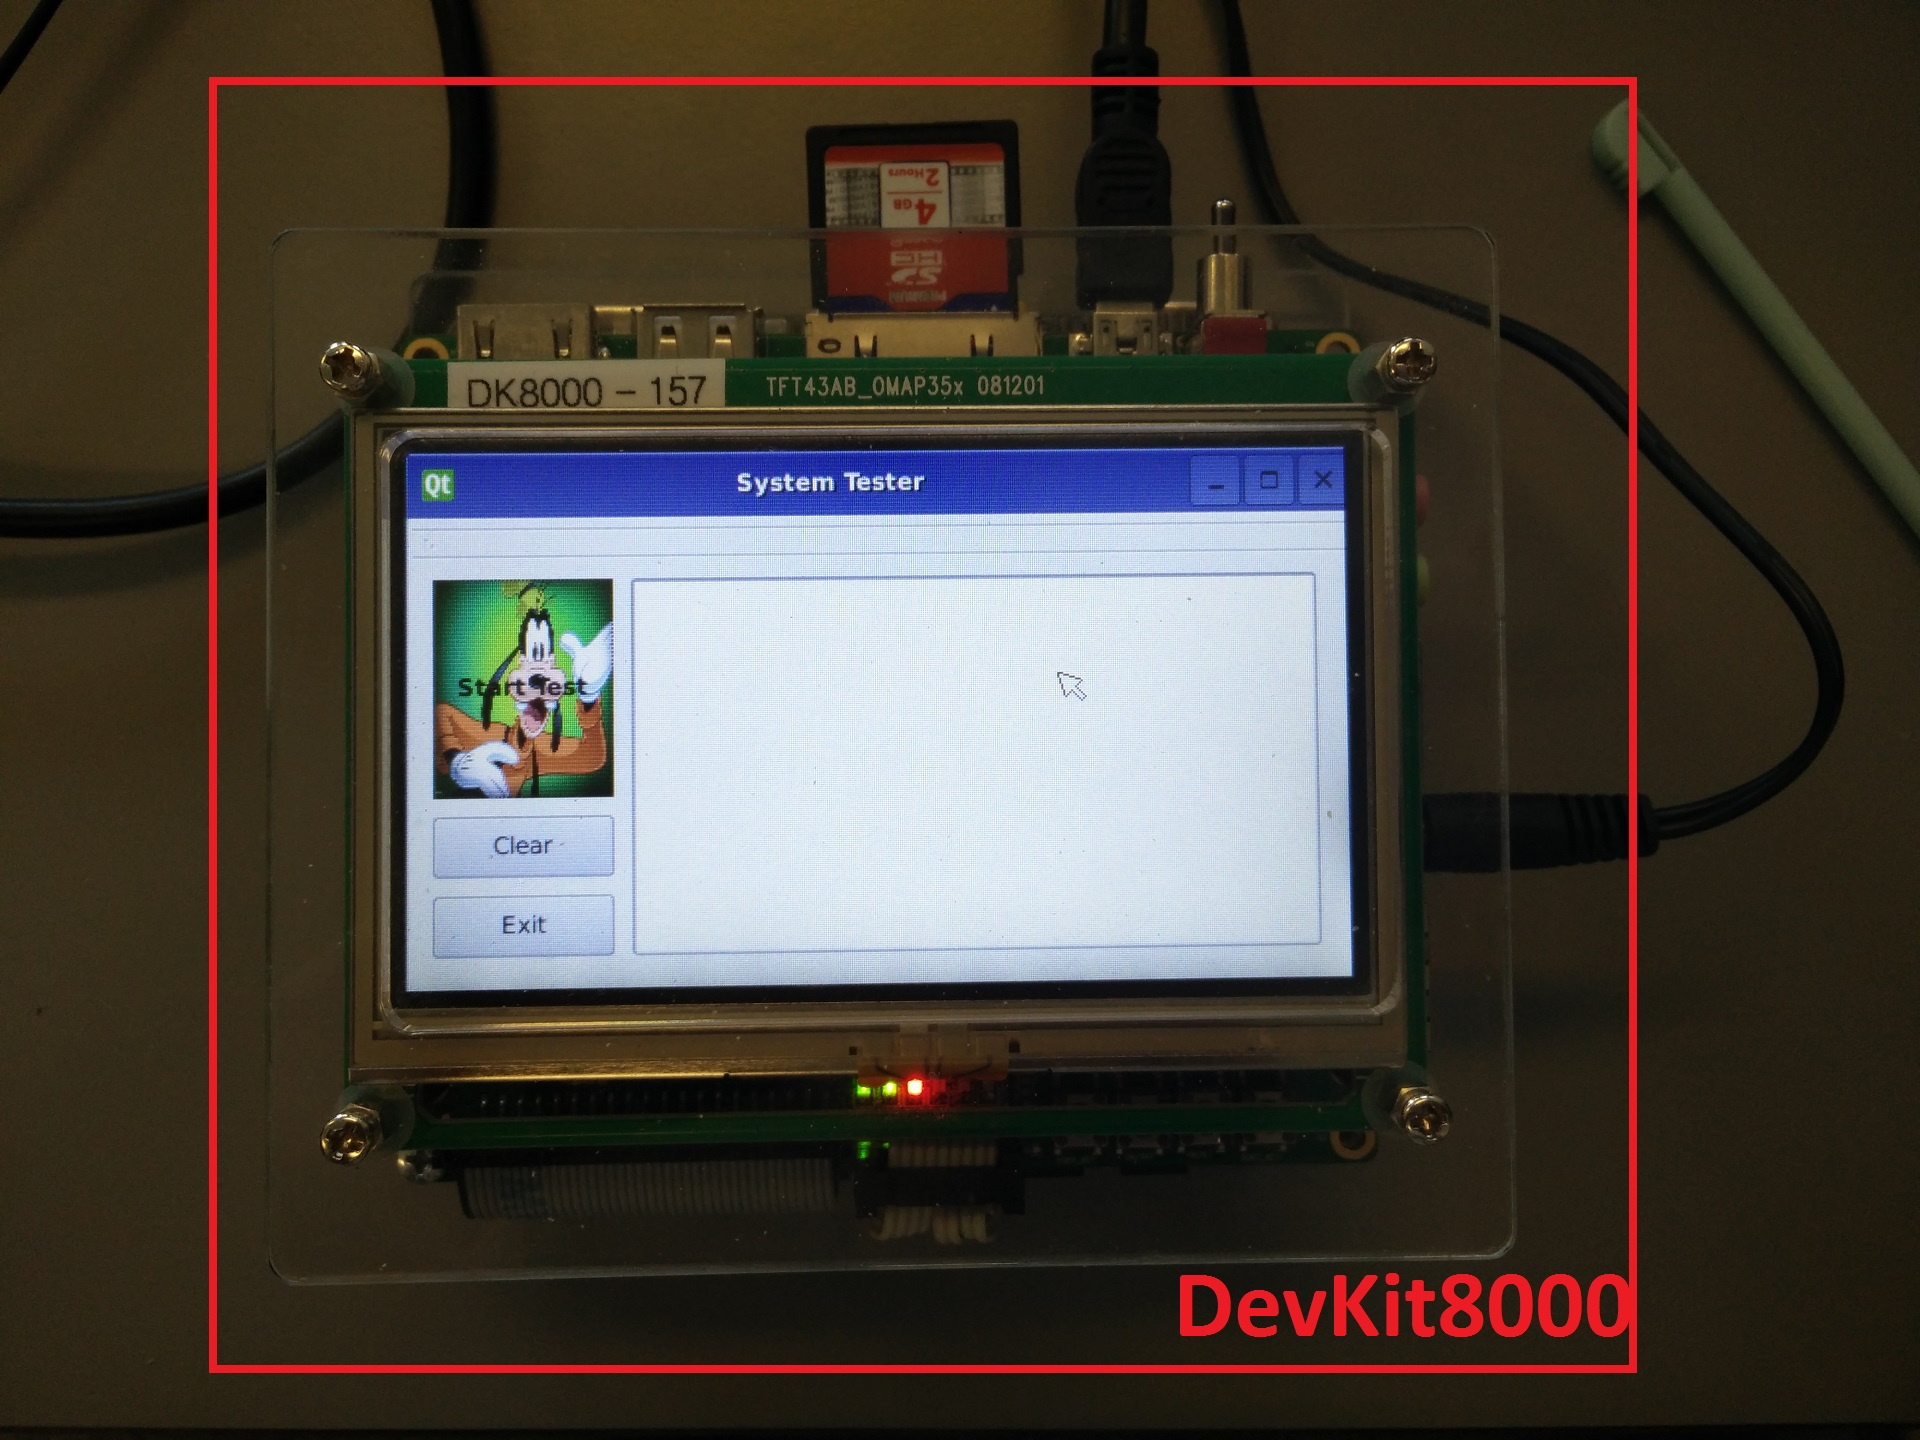
\includegraphics[width=.5\textwidth]{Test/images/GUITest/TestSetup.jpg}
	\caption{Test setup for modultest af brugergrænseflade}
	\label{fig:GUISetup}
\end{figure}

\noindent Test af brugergrænsefladen udføres i tre dele og resultater registreres visuelt. Den første del af testen udføres ved tryk på Start Test-knappen, derefter verificeres det i konsol vinduet at knappen har den ønskede funktionalitet. Den anden del udføres ved tryk på Clear-knappen. Målet ved denne del er at konsol vinduet cleares.
Sidste del af testen udføres ved tryk på Exit-knappen. Målet ved denne del er at programmet lukkes på DevKittet.


\subsubsection{Start Test-knap Test}
I testen trykkes der på knappen "Start Test", og knappens funktion køres i programmet.\newline
 
\noindent\textbf{Forventet resultat:}\newline
\noindent Konsol printer følgende:\newline
Starting System test\newline
Starting SPI Test\newline
Spi Test Successful\newline
Starting I2C Test\newline
I2C Test Successful\newline
Starting Nunchuck Test\newline
Please press the Z button within 6 seconds\newline
Nunchuck Test Successful
\noindent Programmet returnerer til idle-tilstand og konsol vinduet bliver ikke clearet.\newline

\noindent\textbf{Visuelt resultat:}\newline
Som det ses på figur \ref{fig:GUIPrint} bliver det forventet resultat opnået, og konsollen printer som forventet.
Programmet er returneret til idle-tilstand og teksten er ikke blevet clearet. 

\begin{figure}[H]
	\centering
	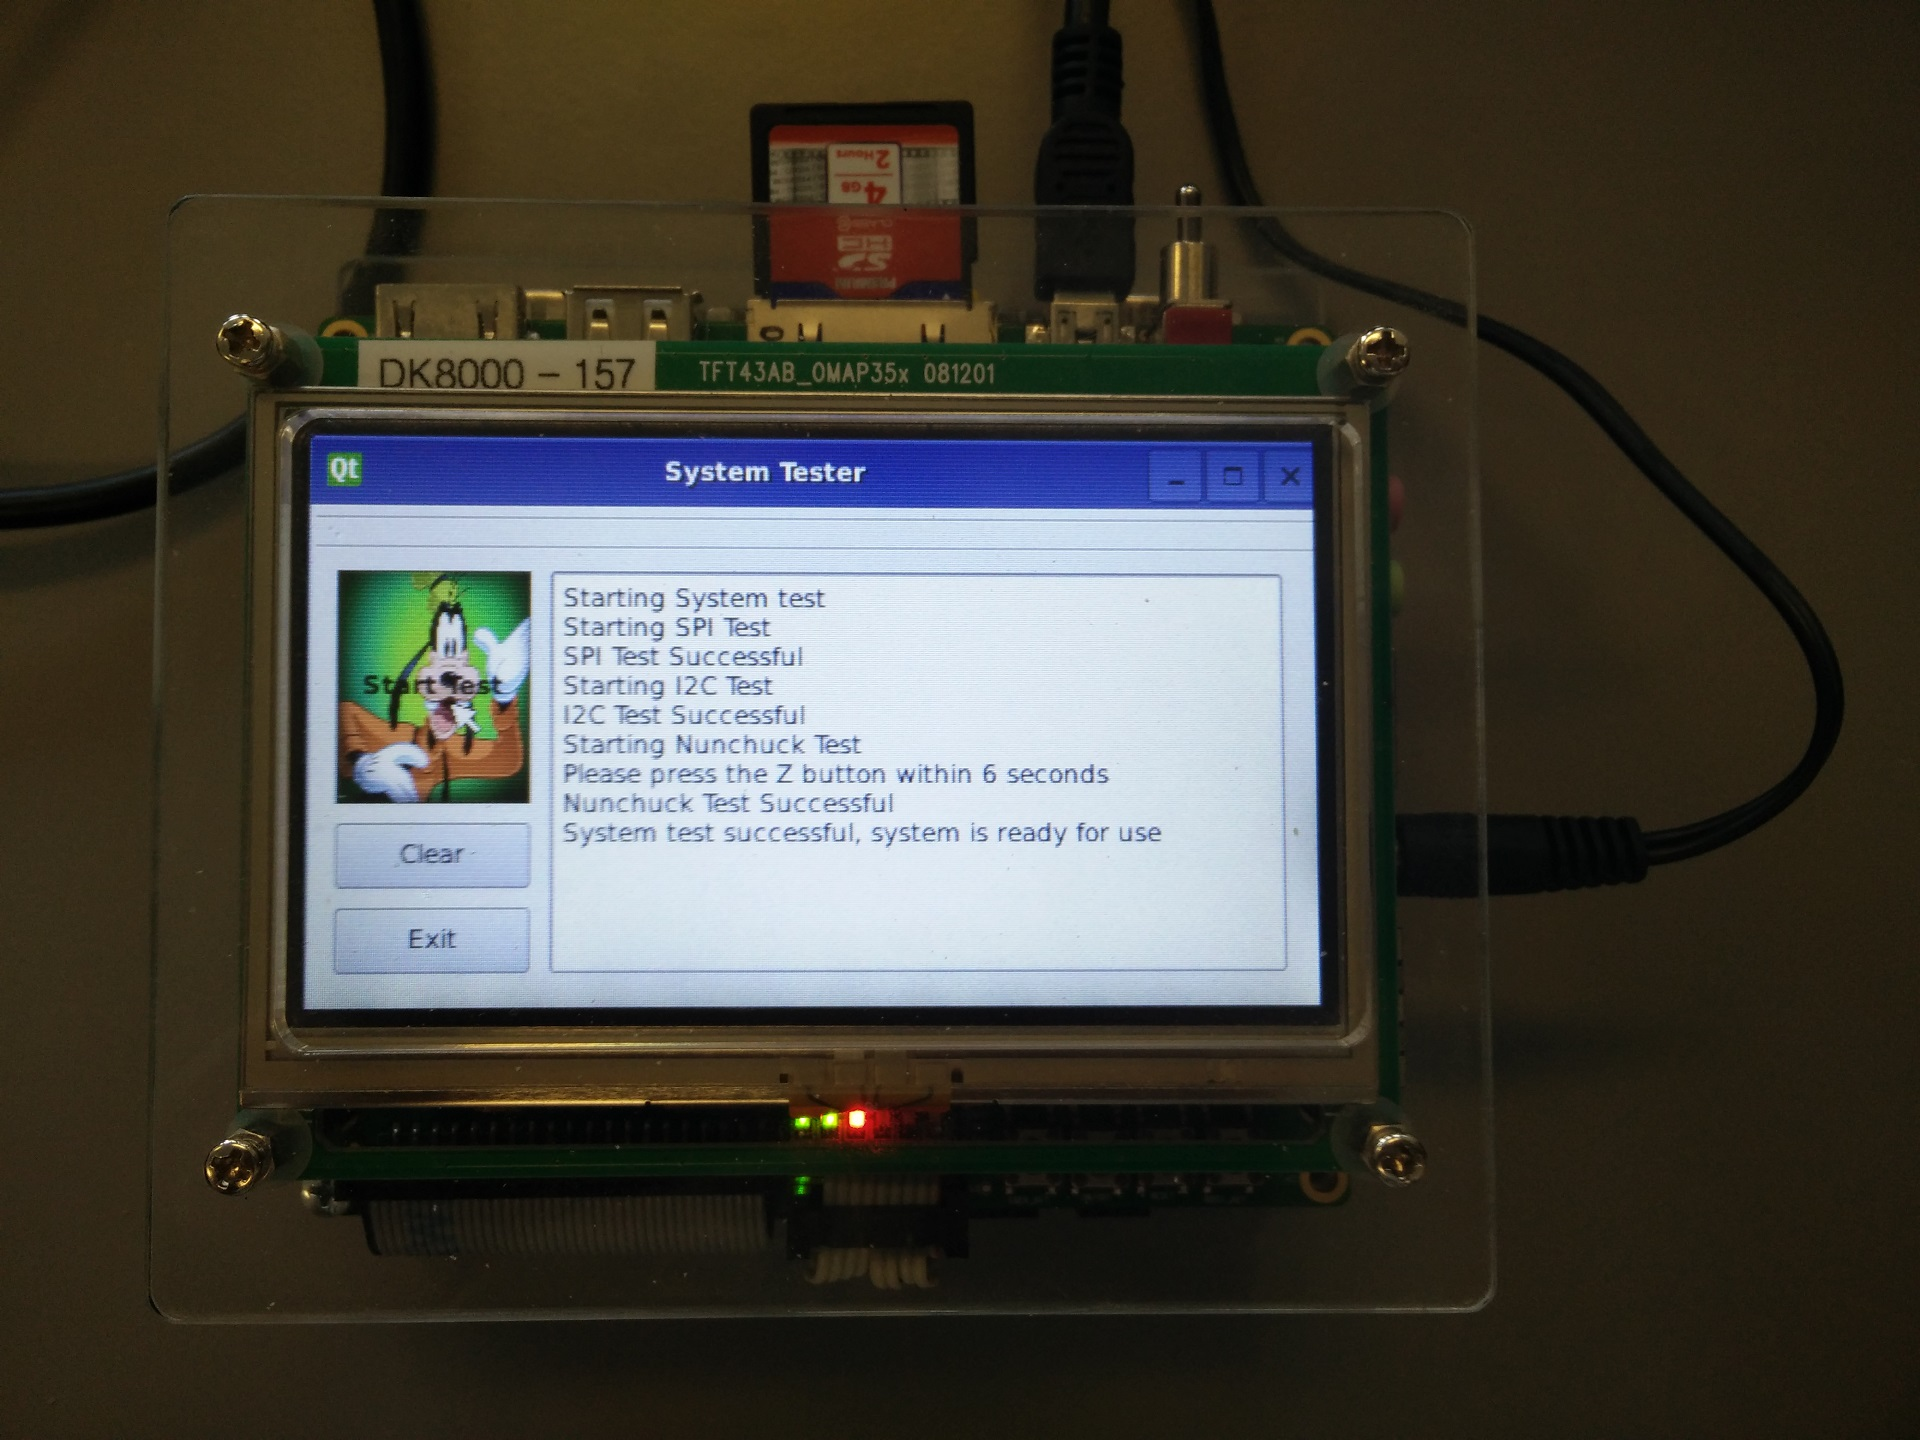
\includegraphics[width=.5\textwidth]{Test/images/GUITest/TestPrint.jpg}
	\caption{Visuel respons af Start Test-knap funktioalitet}
	\label{fig:GUIPrint}
\end{figure}

\subsubsection{Clear-knap Test}
I testen trykkes der på knappen "Clear", og knappens funktion køres i programmet.\newline

\noindent\textbf{Forventet resultat:}\newline
Konsol vinduet, hvor i der er skrevet resultatet fra forrige test, bliver clearet. Programmet returnerer til idle-tilstand.\newline

\noindent\textbf{Visuelt resultat:}\newline
\noindent Som det ses på figur \ref{fig:GUIClear} bliver konsol vinduet clearet og programmet returnerer til idle-tilstand.\newline

\begin{figure}[H]
	\centering
	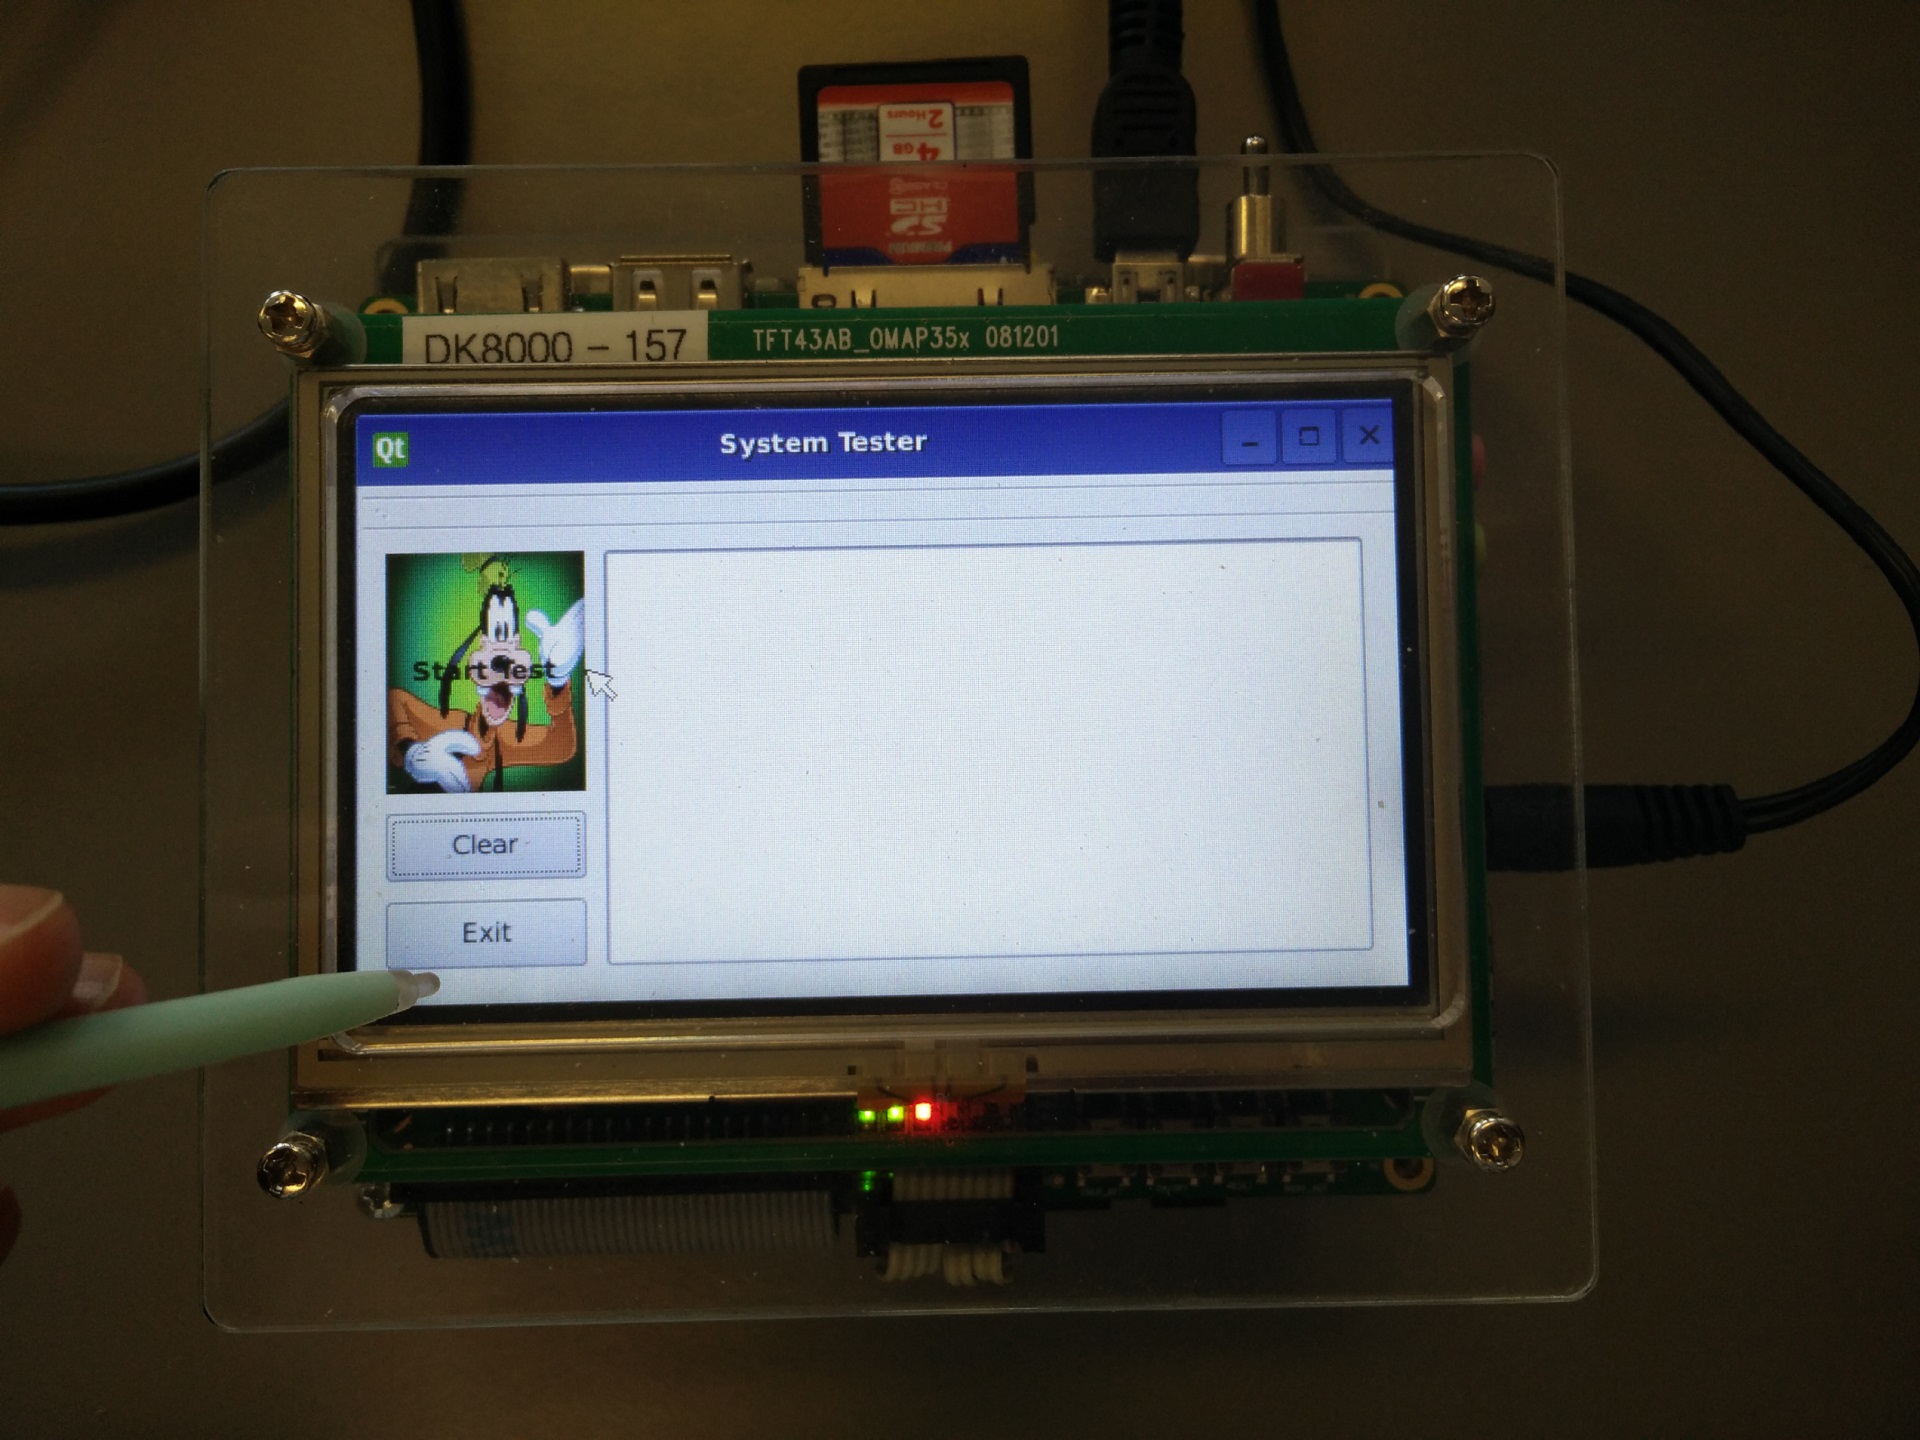
\includegraphics[width=.5\textwidth]{Test/images/GUITest/TestClear.jpg}
	\caption{Visuel respons af Clear-knap funktioalitet}
	\label{fig:GUIClear}
\end{figure}

\subsubsection{Exit-knap Test}
I testen trykkes der på knappen "Exit", og knappens funktion køres i programmet.\newline

\noindent\textbf{Forventet resultat:}\newline
\noindent Programmet lukkes.\newline

\noindent\textbf{Visuelt resultat:}\newline
Som det ses på figur \ref{fig:GUIExit} lukkes programmet.

\begin{figure}[H]
	\centering
	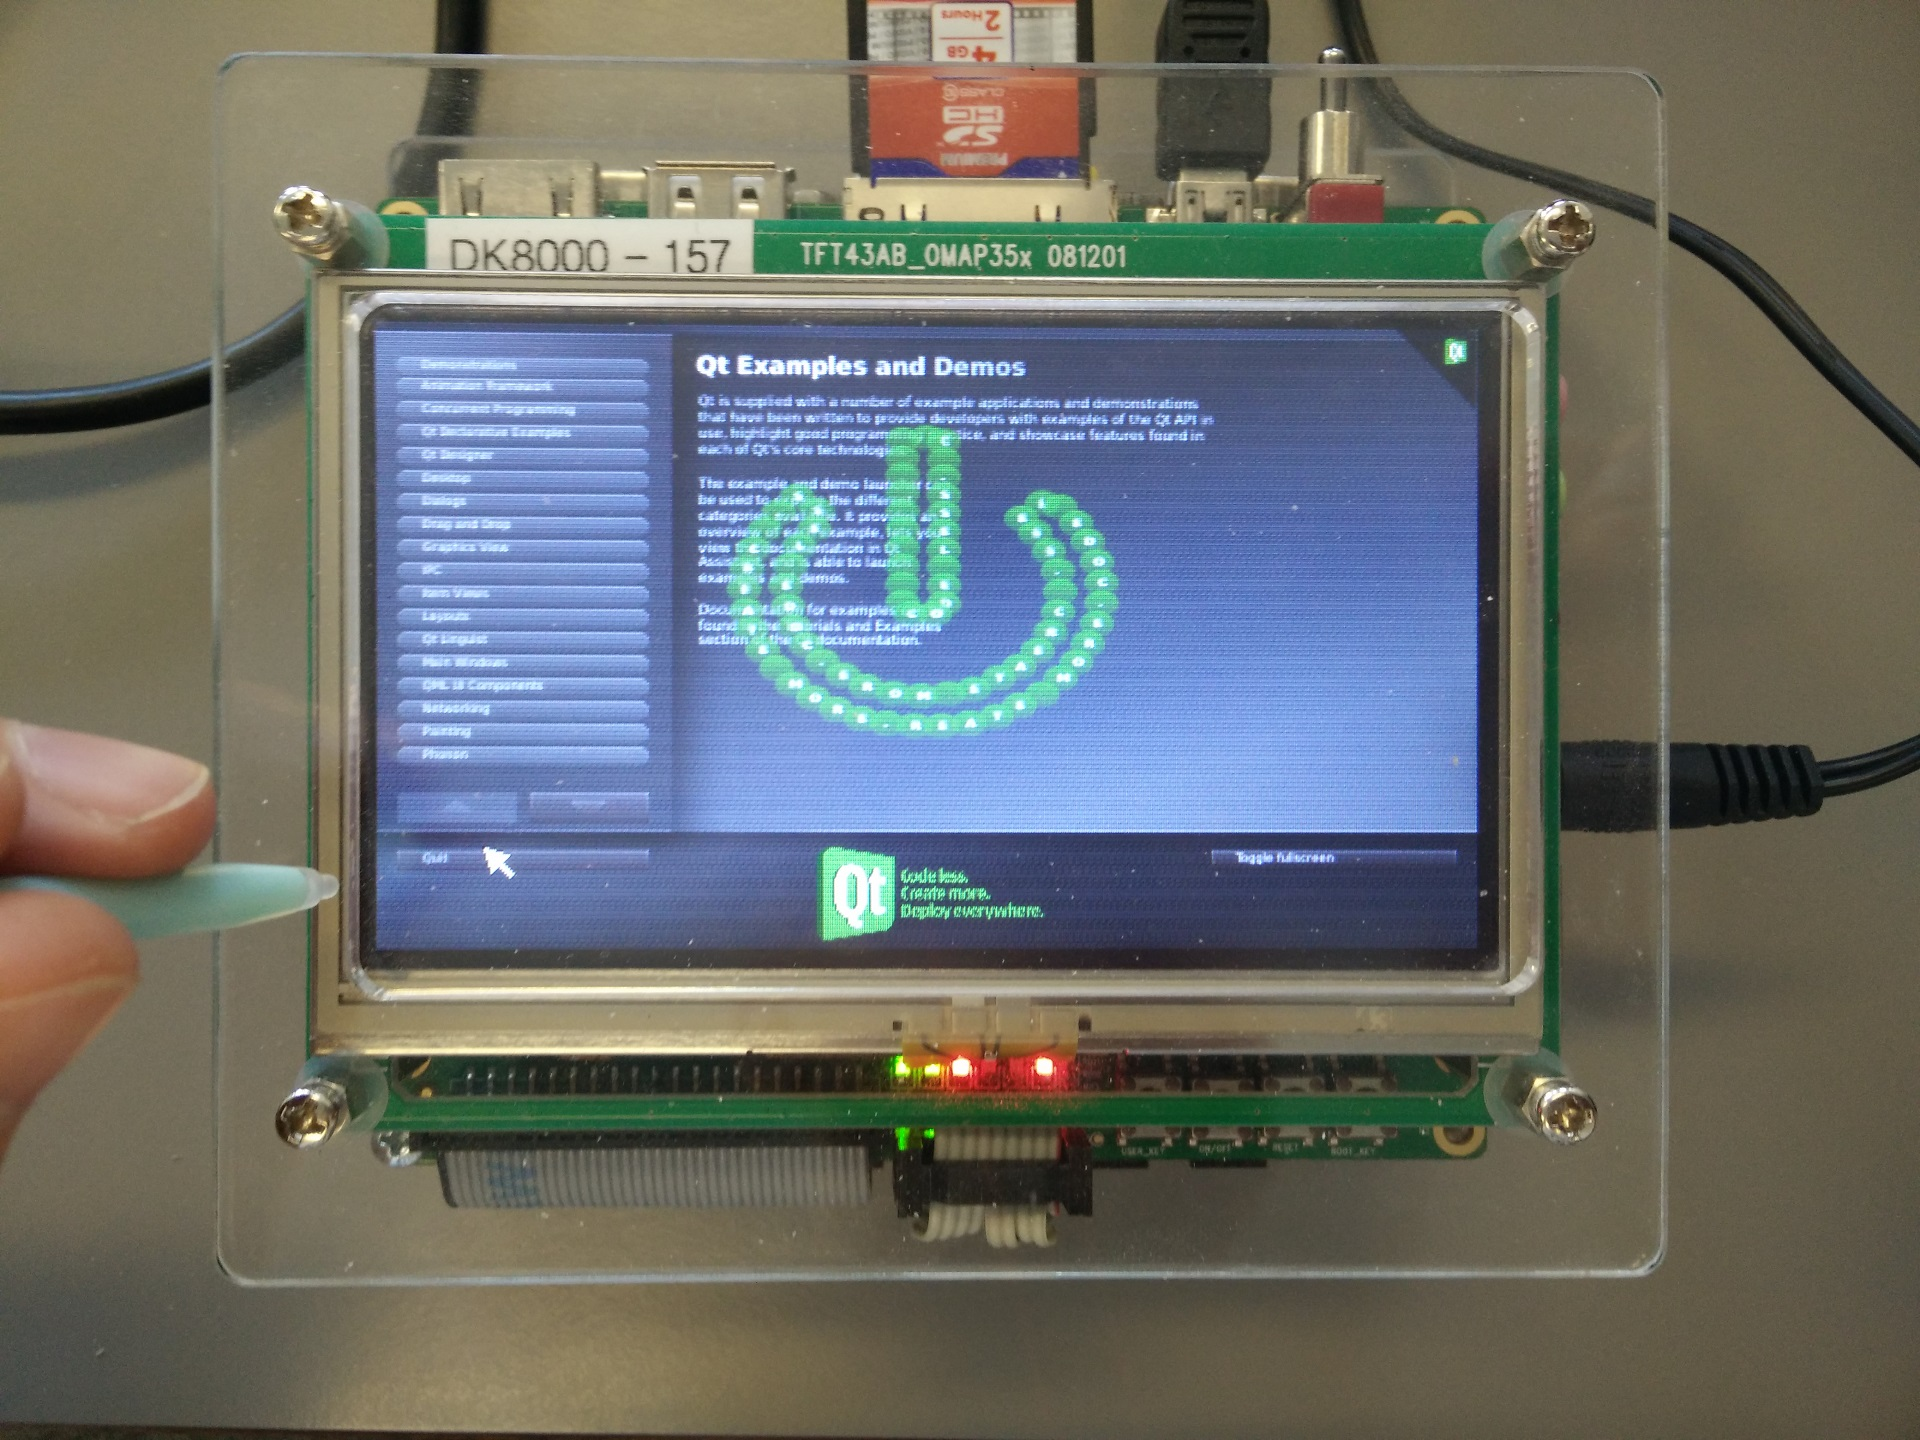
\includegraphics[width=.5\textwidth]{Test/images/GUITest/TestExit.jpg}
	\caption{Visuel respons af Exit-knap funktioalitet}
	\label{fig:GUIExit}
\end{figure}

\section{Hardware}
\subsection{H-bro} 

\textbf{Formål} \newline
Formålet med denne test er at vise at en motor kan styres i begge retninger med H-broen.\newline

\noindent \textbf{Opstilling}

\begin{figure}[H]
	\centering
	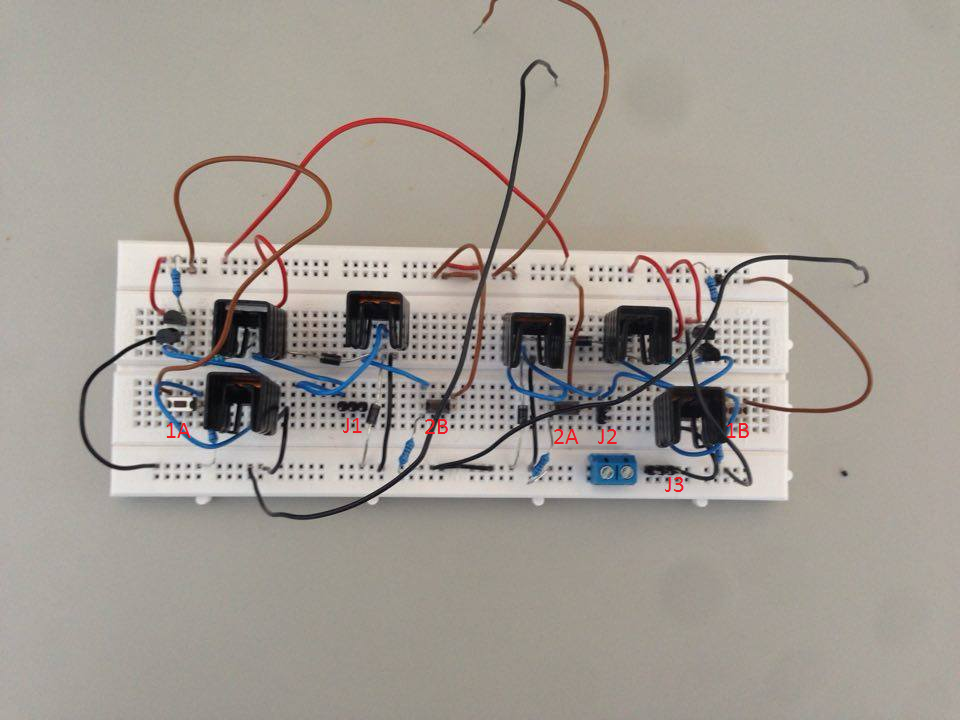
\includegraphics[width=\textwidth]{test/images/testhbroopst}
	\caption{Opstilling af h bro på fumlebræt}
\end{figure}

\begin{itemize}
	\item 	Røde ledninger: 9 V
	\item	Brune ledninger: 5 V
	\item	Sorte ledninger er stel
	\item	Blå ledninger er forbindelser komponenter
	\item	J1 og J2 er output pins 
	\item	J3 er ground
	\item	1a og 2a knapper til at styre motor til højre
	\item	1b og 2b knapper til at styre motor til venstre 	
\end{itemize}

\noindent Til test af H-broens motorstyring i begge retninger blev to oscilloskop kanaler forbundet til output pin J1 og J2, samt oscilloskopene stel til J3. Fumlebrættet forsynes med 9V, 5V og stel fra en spændingskilde. 

\noindent Testen blev udført i to dele. Først testes H-broen i højre omdrejningsretning ved at trykke på 1a og 2a, derefter i venstre omdrejning ved at trykke 1b og 2b. \newline

\noindent \textbf{Forventet resultat} \newline
At når der blev trykket på knap 1a og 2a vil den ene kurv gå høj og den anden vil for blive lav
At når der blev trykket på knap 1b og 2b vil den anden kurv gå høj og den først vil for blive lav.
\\
\\

\textbf{Opnået resultat}
\begin{figure}[H]
	\centering
	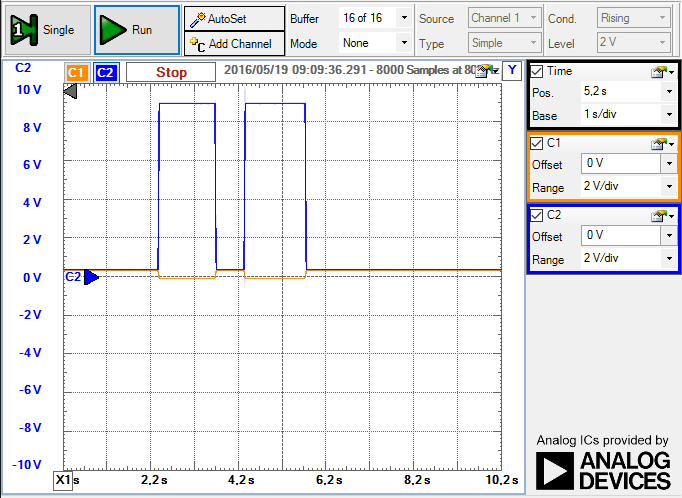
\includegraphics[width=\textwidth]{test/images/hbromob}
	\caption{Modultest for H-bro, blå går høj}
		\label{figure:hbrob}
	
\end{figure}
\begin{figure}[H]
	\centering
	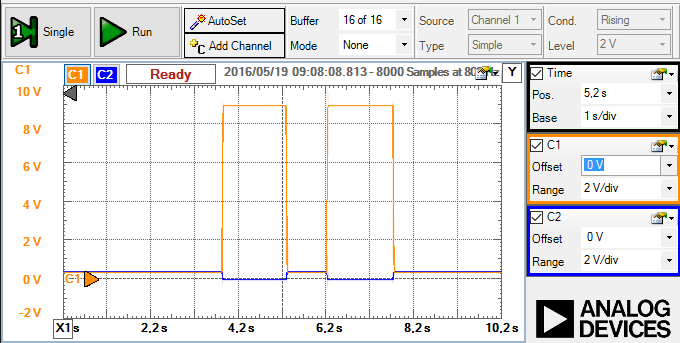
\includegraphics[width=\textwidth]{test/images/hbromoo}
	\caption{Modultest for H-bro, orange går høj}
	\label{figure:hbroo}
	
\end{figure}
 Som det fremgår på figur \ref{figure:hbrob}, kan man se at, i det der bliver åbnet for at motor kan køre i den ene retning, så stiger den blå op til 9V fordi nu har den fået forbindelse til ground og fået forbindelse til de 9V. Hvor samtidigt at blå går højt, så går den orange lavere, for nu trækker den blå alt spændingen. Det samme sker når man åbner op for at den kan løbe spændingen kan løbe den anden vej, som ses på firgur \ref{figure: hbroo}, i stedet for at det er den blå som går høj, er det den orange som går høj. Med det kan man se at motor kan køre i begge retninger uden problemer.
 Der er blevet valgt at der ikke tages billede af at motoren køre, for man ikke se på et billede hvilken vej den køre og overhovedet den køre. Der ses også på figur\ref{figure:hbrob} og figur \ref{figure:hbroo} at der noget støj, når orange/blå går højt, men det er ikke noget som kommer til at påvirker vores styring af motoren

Man kan også på figur se at når den orange/blå går høj, så stiger den meget hurtig, grunden til den gør det var på grund af at, der er blevet sat de to transistor ind, får p mosfet, som gør at den bliver opladt hurtigere, end den ellers ville på grund af der sidder en form for kondensatorer inde i den mosfet, som skal have hjælp med at bliv opladt. Det hjælp kommer fra de transistor som er blevet sat ind før Mosfeten.  

\subsection{detektor}

\textbf{Formål}
\\ Formålet med denne test er at vise at motoren ikke kan køre ud over to fast satte værdier.\\
\\
\textbf{Overordnet opstilling}
\begin{figure}[H]
	\centering
	\includegraphics[width=\textwidth]{test/images/ModultestADC/opstilADC}
	\caption{opstilling af test for detektor}
\end{figure}


\begin{itemize}
	\item Rød firekant 1 er potentiometer
	\item	Rød firekant 2 er h-broen på print
	\item	Rød firekant 3 ”PSoC 1”
	\item	Rød firekant 4 er wii nunchuck
	\item	Rød firekant 5 er ”PSoC 0” hvor der 3 ledninger(lilla, blå og orange) som går til devkit 
	\item Rød firekant 6 hvor der sidder pull up modstande til kommunikationen mellem ”PSoC 1” og ”PSoC 0”
	\item	sort ledning går til ground 
	\item	gul ledning er data mellem de forskellige module
	\item grøn ledning er klokken
	\item rød ledningen er spænding til h -bro
	
\end{itemize}
For at teste om motor kunne køre i begge retninger når den er i mellem 900mV og 2000mV og når den kommer over 2000mV eller under 900mV skal den ikke kunne køre i en af retningerne.
For at tjekke hvilken værdi som blev brugt, blev der sat en analog discovery på potentiometeret og på ADC, blev der debugget og så for at tjekke om motoren kun kunne køre i en retning blev det en visueltest. \\
\\
Første del af testen består i at tjekke om motoren kan kun køre mod venstre, når potentiometeret er drejet til en værdi under 900mV. Hvor der blev set på hvilken værdi potentiometer gav og hvad ADC’en fik og en visueltest af om motoren kun kunne køre i en retning.\\
Andel del af testen består i at tjekke om motoren kunne køre begge vej, når potentiometeret er drejet til en værdi mellem 900mV og 2000mV. Hvor der blev set på hvilken værdi potentiometer gav og hvad ADC’en fik og en visueltest af om motoren kun kunne køre i begge retning.\\
Tredje del består i at tjekke om motoren kan kun køre mod højre, når potentiometeret er drejet til en værdi over 2000mV. Hvor der blev set på hvilken værdi potentiometer gav og hvad ADC’en fik og en visueltest af om motoren kun kunne køre i den anden retning.\\
\\
\textbf{Forventet resultat }
\\Første del: at når der en værdi under 900mV bliver sendt ind, vil motoren kun kunne køre mod venstre.\\
Anden del: at når der en værdi mellem 900mV og 2000mV bliver sendt ind, vil motoren kunne køre i begge retninger.\\
Tredje del: at når der en værdi over 2000mV bliver sendt ind, vil motoren kun kunne køre mod højre.

\textbf{Opnået resultat}
\begin{figure}[H]
	\centering
	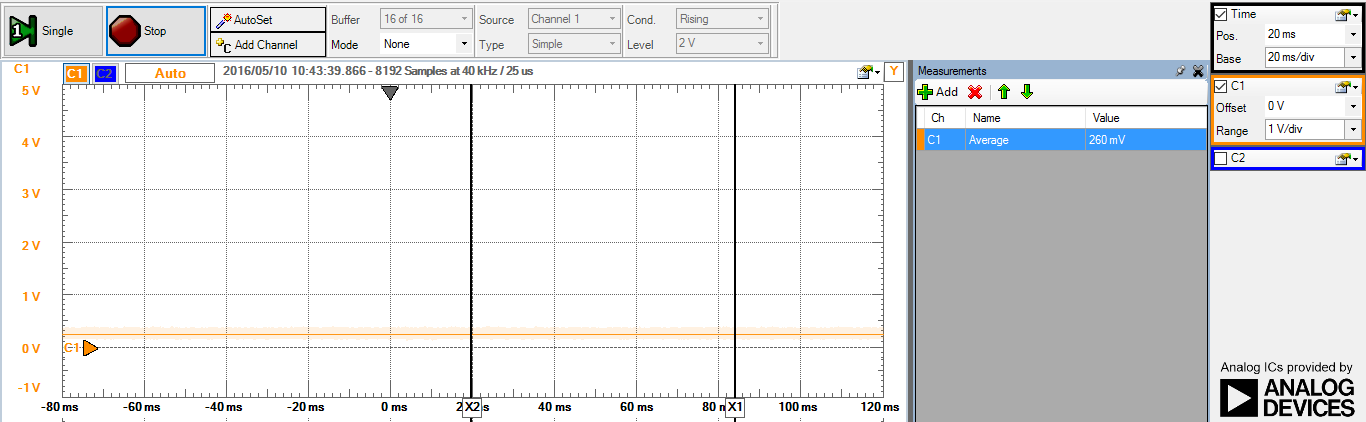
\includegraphics[width=\textwidth]{test/images/ModultestADC/260mVanalog}
	\caption{måleresultat fra analog Discovery, ved først del af test}
	\label{figure:analoglav}
\end{figure}
\begin{figure}[H]
	\centering
	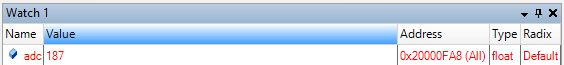
\includegraphics[width=\textwidth]{test/images/ModultestADC/nedDebug}
	\caption{måleresultat fra ADC, ved først del af test}
	\label{figure: ADClav}
\end{figure}
Først del: Som det fremgår på figur \ref{fig:analoglav} bliver der sendt fra potentiometeret  en spænding på 260mV og på firgur \ref{fig:ADClav} kan man se at ADC’en modtog en værdi på 187mV, man skal huske på at der en forskel på 1.515 i mellem potentiometeret og ADC \textbf{\#ref Reference til DesignOgImplementering }. 
Som forventet kunne motoren kun køre mod venstre\\
\begin{figure}[H]
	\centering
	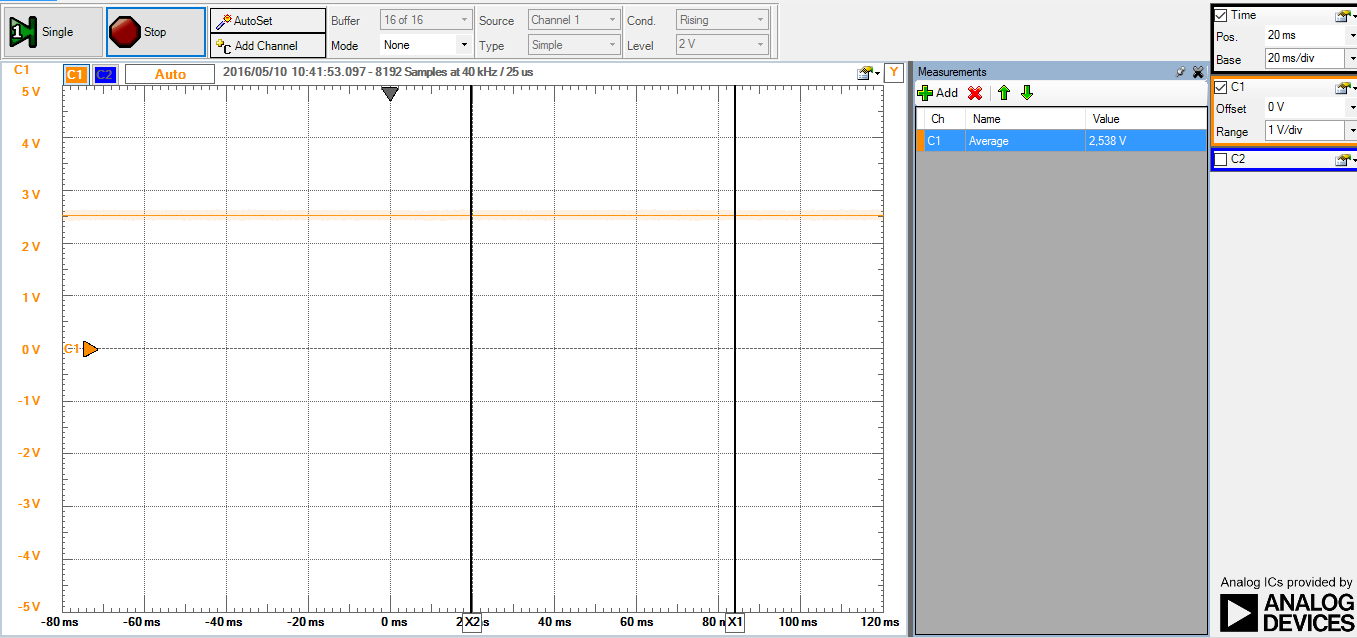
\includegraphics[width=\textwidth]{test/images/ModultestADC/2538Vanalog}
	\caption{måleresultat fra analog Discovery, ved anden del af test}
	\label{figure:analogmid}
\end{figure}
\begin{figure}[H]
	\centering
	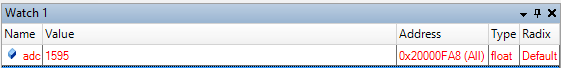
\includegraphics[width=\textwidth]{test/images/ModultestADC/mellemDebug}
	\caption{måleresultat fra ADC, ved anden del af test}
	\label{figure: ADCmid}
\end{figure}
Anden del: Som det fremgår på figur \ref{fig:analogmid}  bliver der sendt fra potentiometeret en spænding på 2538mV og på firgur \ref{fig:ADCmid}  kan man se at ADC’en modtog en værdi på 1595mV, man skal huske på at der en forskel på 1.515 i mellem potentiometeret og ADC \textbf{\#ref Reference til DesignOgImplementering }. 
Som forventet kunne motoren kun køre i begge retninger.\\


\begin{figure}[H]
	\centering
	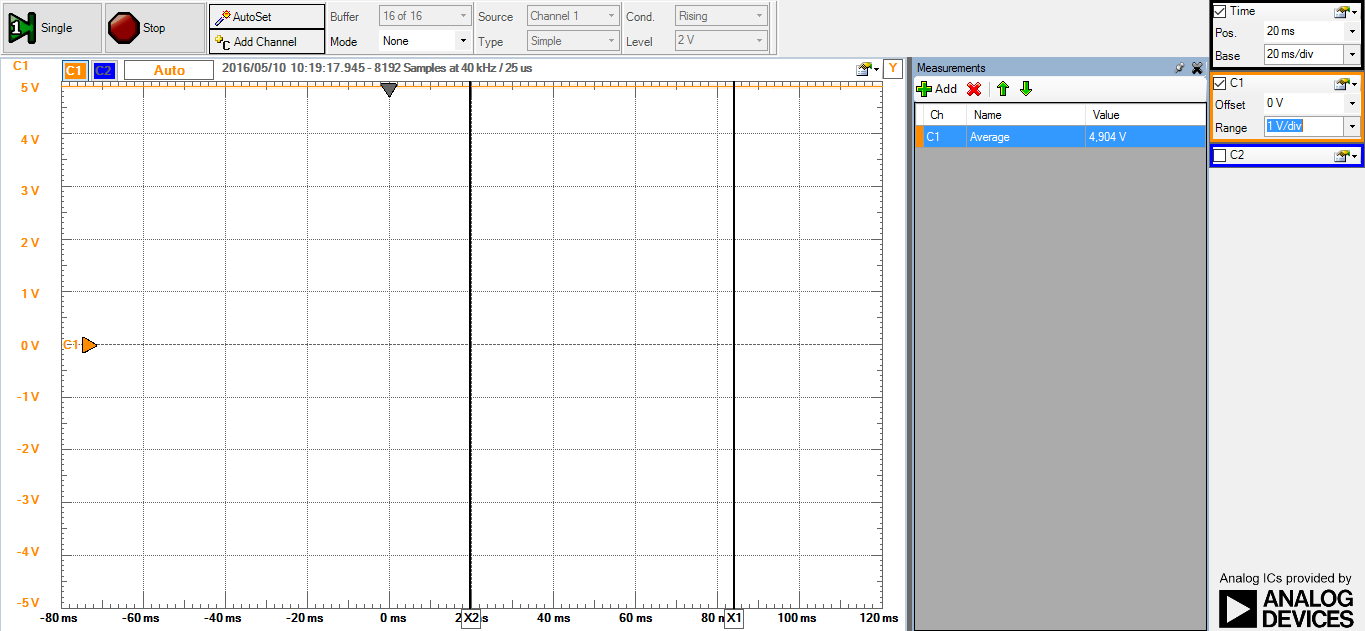
\includegraphics[width=\textwidth]{test/images/ModultestADC/4904mVanalog}
	\caption{måleresultat fra analog Discovery, ved trejde del af test}
	\label{figure:analoghoj}
\end{figure}
\begin{figure}[H]
	\centering
	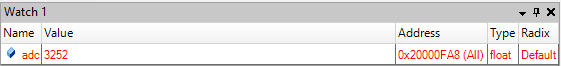
\includegraphics[width=\textwidth]{test/images/ModultestADC/opDebug}
	\caption{måleresultat fra ADC, ved trejde del af test}
	\label{figure: ADChoj}
\end{figure}
Tredje del: Som det fremgår på figur \ref{fig:analoghoj} bliver der sendt fra potentiometeret en spænding på 4909mV og på firgur \ref{fig:ADChoj}  kan man se at ADC’en modtog en værdi på 3252mV, man skal huske på at der en forskel på 1.515 i mellem potentiometeret og ADC \textbf{\#ref Reference til DesignOgImplementering }. 
Som forventet kunne motoren kun køre mod højre.


\subsection{Rotationsdetektor}
Der er udført en række modultests af rotationsdetektoren. Først er der en beskrivelse af testen, der skulle teste de forskellige dele i rotationsdetektorkredsløbet, både mens fotodioden modtager et lyssignal fra LED'en, og når den ikke gør. Herefter følger en beskrivelse af modultesten af det båndpasfilter, der indgår i rotationsdetektoren og til sidst er der en beskrivelse af modultesten af motorens PWM-signal. 

På figur \ref{fig:målepunkter} ses, hvor der er målt for at teste rotationsdetektoren. 

\begin{figure}[H]
	\centering
	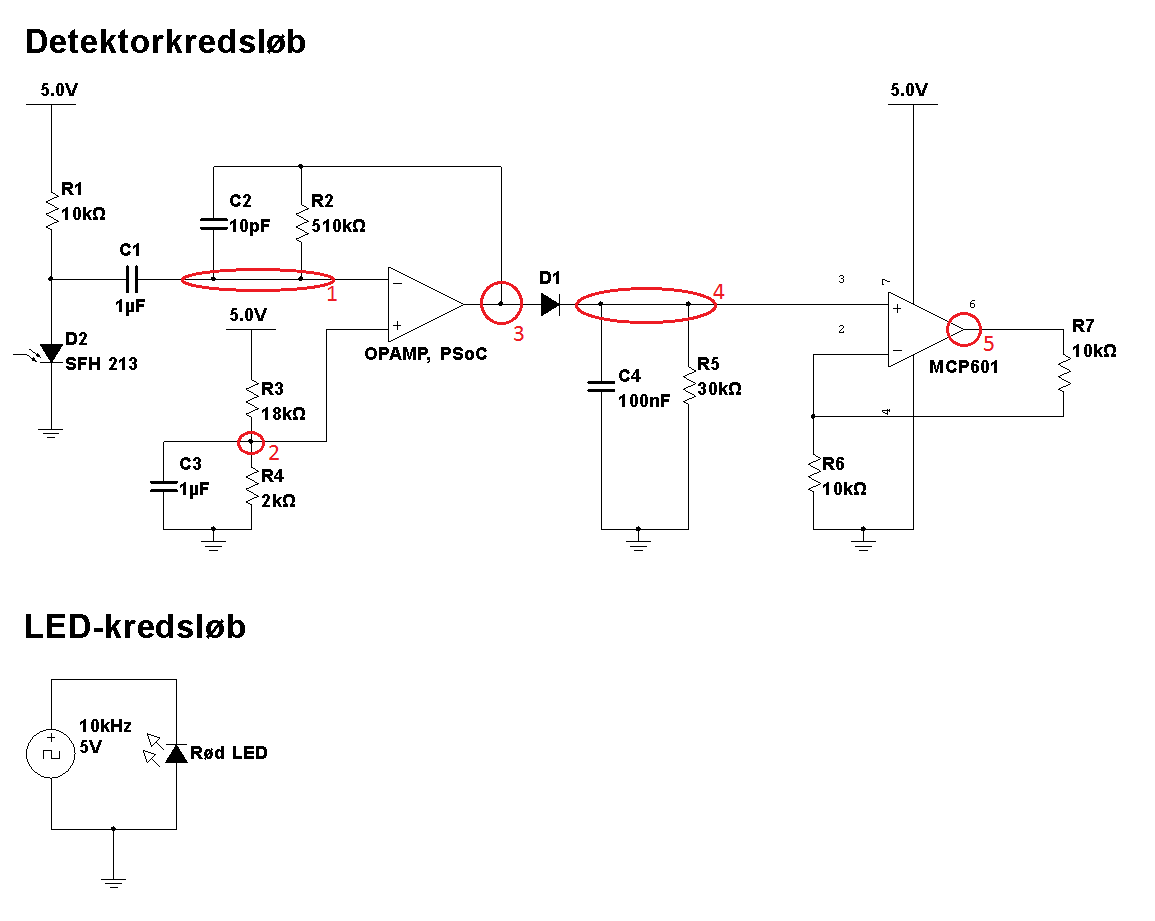
\includegraphics[width=\textwidth]{Test/images/rotationsdetektor_maalepunkter}
	\caption{Målepunkter på rotationsdetektor}
	\label{fig:målepunkter}
\end{figure}

I tabel \ref{dioderIkkeSe} ses resultaterne fra modultesten af rotationsdetektoren, når fotodioden ikke får noget lyssignal. Det ses, at det virtuelle nul fra spændingsdeleren ligger på 0,4V, og at forstærkeren fordobler signalet, hvilket var meningen. 

\begin{table}[H]
	\centering
	\begin{tabular}{|l|l|c|c|}
		\hline
		\textbf{Knudepunkt}		& \textbf{Målested}       & \textbf{Forventet resultat} & \textbf{Målt resultat} \\ \hline
		1						& Virtuelt 0              & 0,5V                        & 0,4V                   \\ \hline
		2						& Spændingsdeler          & 0,5V                        & 0,45V                  \\ \hline
		3						& Udgang på OpAmp på PSoC & 0,5V                        & 0,4V                   \\ \hline
		4 						& Envelope detector       & 0,5V                        & 0,4V                   \\ \hline
		5 						& Udgang på forstærker    & 1V                          & 0,85V                  \\ \hline
	\end{tabular}
	\caption{Modultest af rotationsdetektor, når fotodioden ikke modtager lyssignal fra LED}
	\label{dioderIkkeSe}
\end{table}

I tabel \ref{dioderSe} ses resultaterne fra modultesten af rotationsdetektoren, når fotodioden får lyssignal fra LED'en. Her ses det, at der igen er 0,4V, der hvor det var meningen, der skulle være 0,5V, så det er fint. Det ses også, at der er et PWM-signal på udgangen af PSoC'ens operationsforstærker og forstærkeren forstærker signalet, som ønsket. 

\begin{table}[H]
	\centering
	\begin{tabular}{|l|c|c|}
		\hline
		\textbf{Sted}           & \textbf{Forventet resultat} & \textbf{Målt resultat} \\ \hline
		Virtuelt 0              & 0,5V                        & 0,4V                   \\ \hline
		Spændingsdeler          & 0,5V                        & 0,45V                  \\ \hline
		Udgang på OpAmp på PSoC & PWM, 0-5V                   & PWM, 0-4V              \\ \hline
		Envelope detector       & \multicolumn{1}{l|}{}       & 3,7V                   \\ \hline
		Udgang på forstærker    & \multicolumn{1}{l|}{}       & 4,7V                   \\ \hline
	\end{tabular}
	\caption{Modultest af rotationsdetektor, når fotodioden modtager lyssignal fra LED}
	\label{dioderSe}
\end{table}

I tabel \ref{forstaerkerudgang} ses resultaterne fra modultesten af båndpasfilteret. 

\begin{table}[H]
	\centering
	\begin{tabular}{|l|c|c|}
		\hline
		\textbf{PWM-værdi} & \textbf{Forventet værdi} & \textbf{Målt værdi} \\ \hline
		40kHz              & \multicolumn{1}{l|}{}    & 3V                  \\ \hline
		29kHz              & \multicolumn{1}{l|}{}    & 3,9V                \\ \hline
		10kHz              & \multicolumn{1}{l|}{}    & 4,7V                \\ \hline
		10Hz               & \multicolumn{1}{l|}{}    & -                   \\ \hline
		5V (lyser LED?)    & Ja                       & Ja                  \\ \hline
	\end{tabular}
	\caption{Modultest af forstærkerudgangen}
	\label{table:forstaerkerudgang}
\end{table}

Afskæringsfrekvenserne for båndpasfilteret ligger på 15,9Hz og 31,2kHz, så hvis båndpasfilteret skulle være helt optimalt skulle alt, der ligger udenfor disse frekvenser dæmpes fuldstændig. Det ses dog i tabel \ref{forstaerkerudgang}, at det ikke helt er tilfældet. Ved 40kHz er signalet dæmpet til 3V, og ved 10kHz lader filteret alt gå igennem. Ved 10 Hz ses det, at signalet dæmpes, men der forekommer også mange spikes, som forstyrrer signalet. Derfor er der ikke indsat et tal i tabellen. 

\section{Integrationtest - Use case 2}
For at verificere at use case 2 fungerer når det sammensættes til en enkelt enhed, er der lavet en integrationstest. Testen er lavet ud fra et 'black-box' princip, hvilket vil sige, at der kun evalueres ud fra systemets funktionalitet, og ikke på den interne struktur.
Testen udføres ved, at klikke på 'Start-test', og bagefter observeres udskriften på terminal-vinduet på brugergrænsefladen. På figur \ref{figure:IntegrationstestOpstilling} ses opstillingen for integrationstesten.

\begin{figure}[H]
	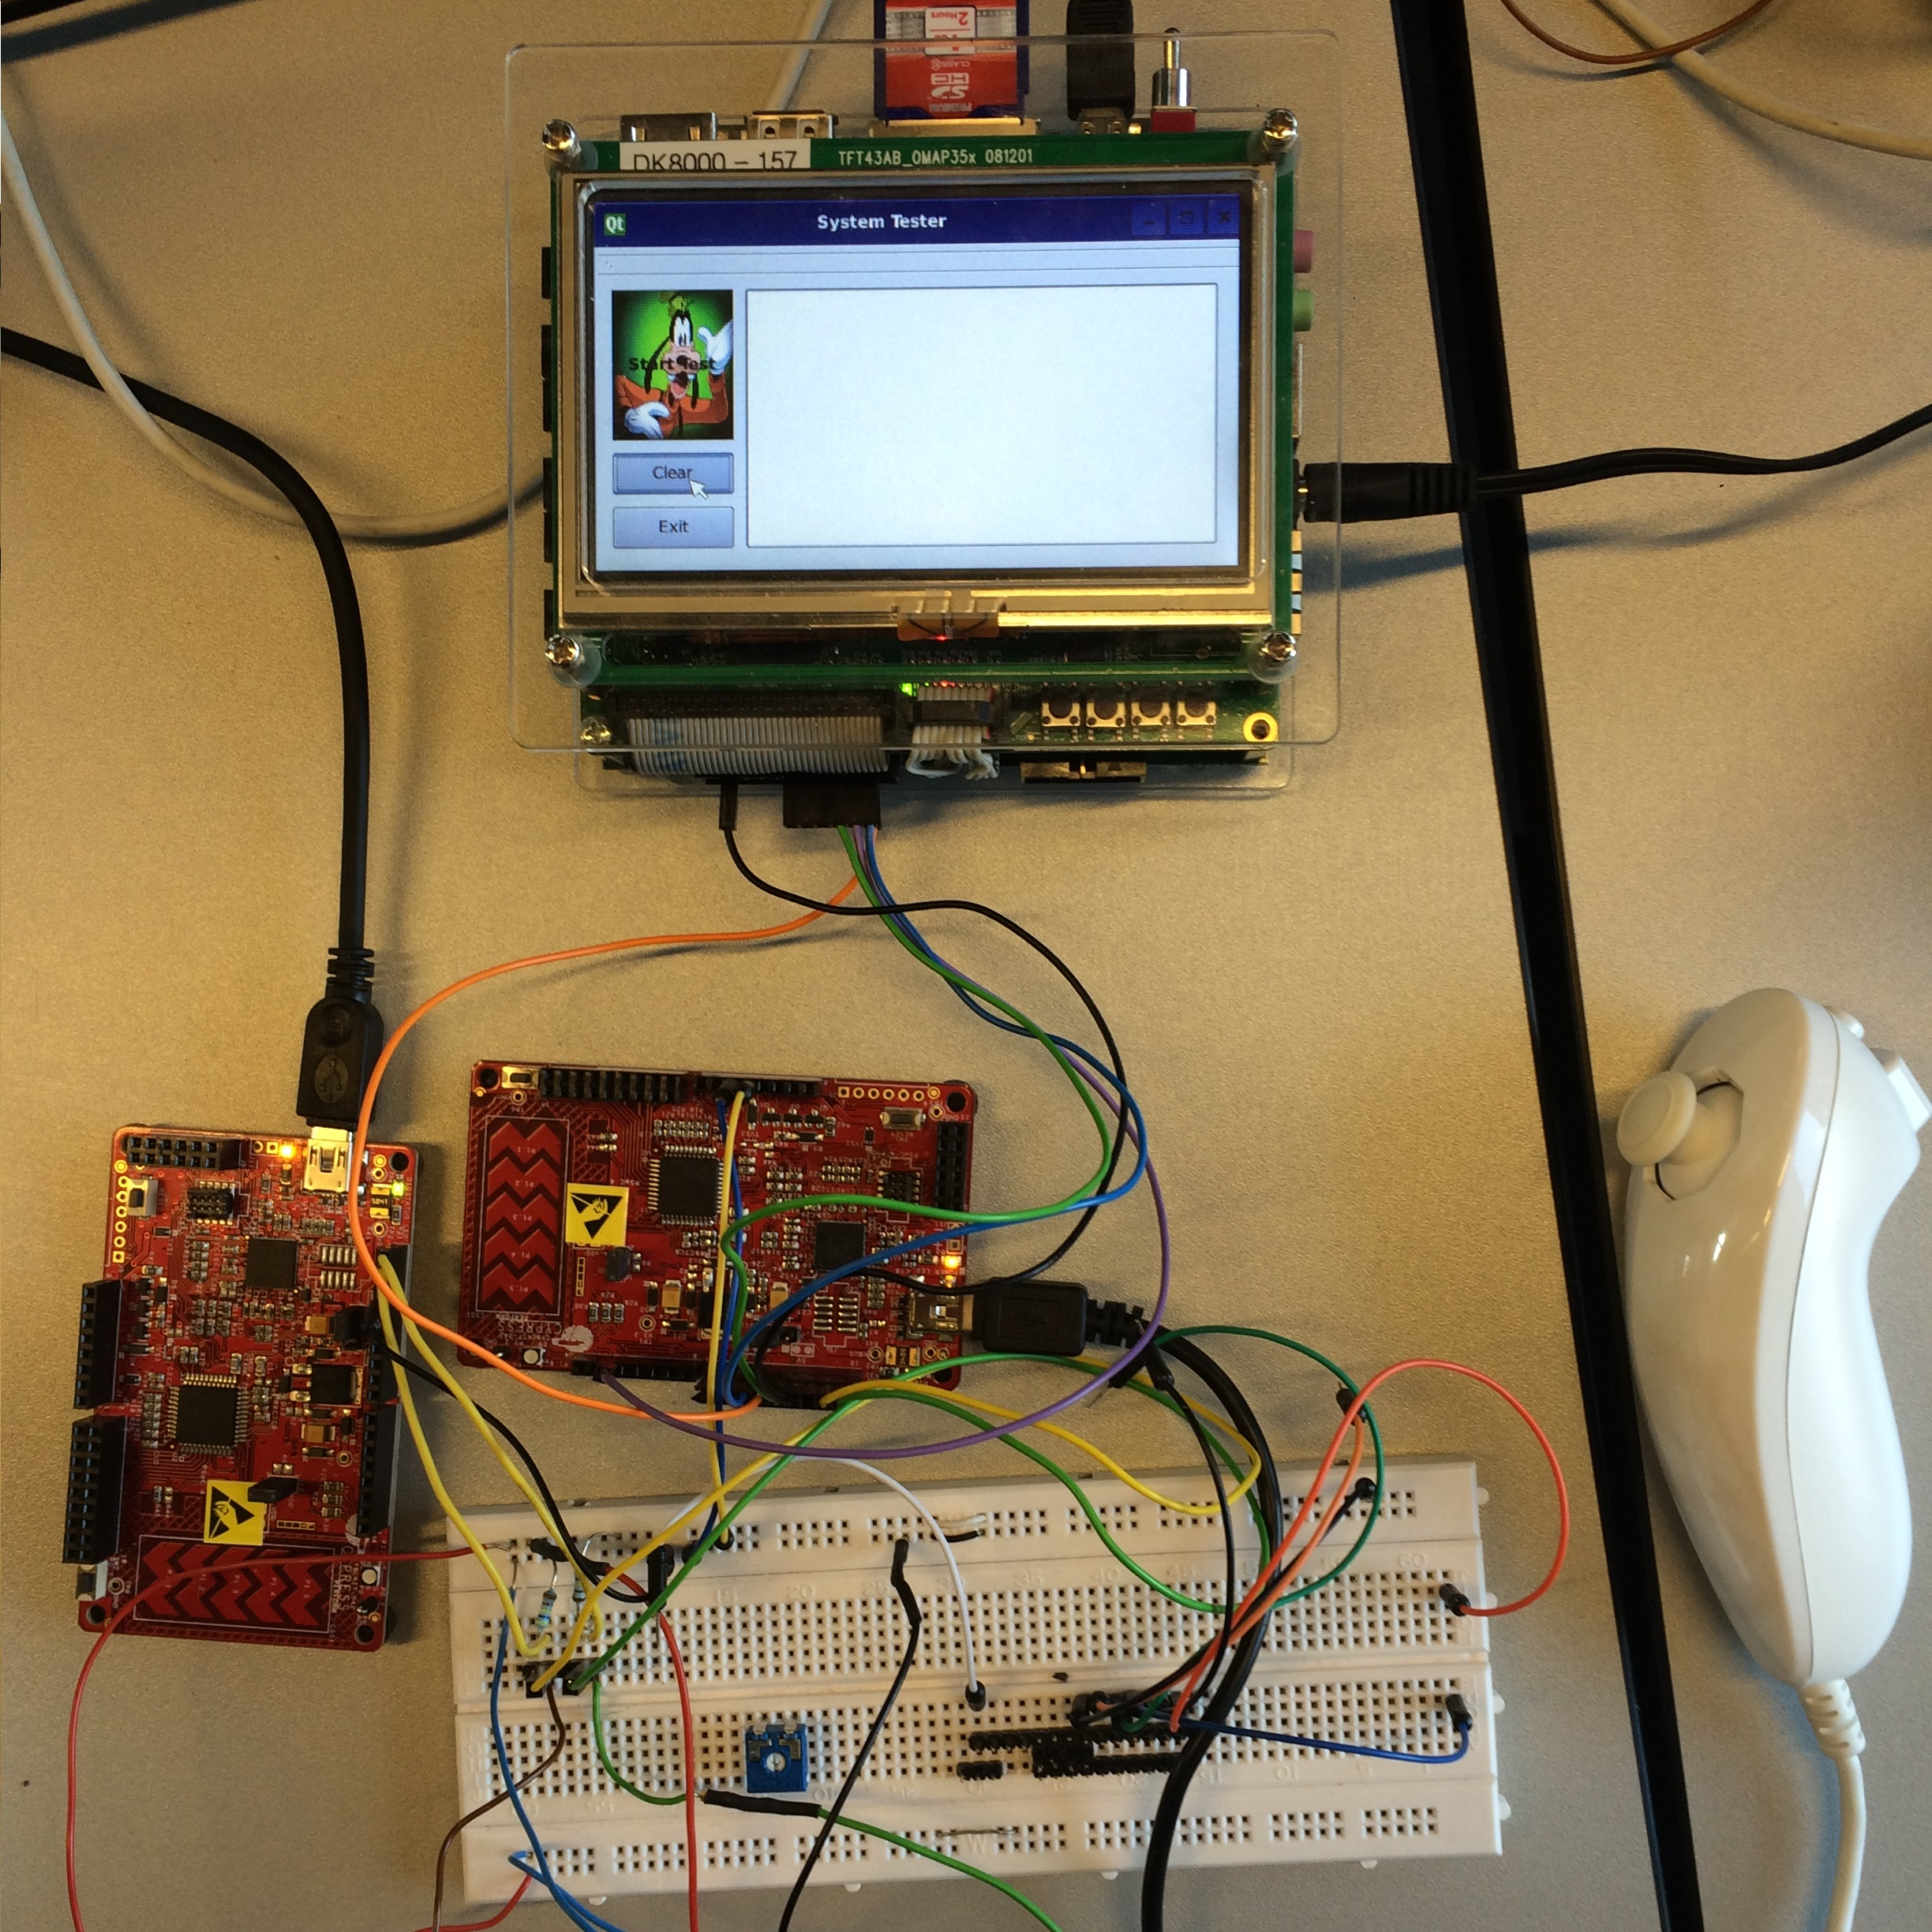
\includegraphics[width=\textwidth]{Test/images/IntegrationstestProtokoller/opstilling}
	\caption{Integrationstest opstilling}
	\label{figure:IntegrationstestOpstilling}
\end{figure}

Opstillingen viser, at Nunchuck'en og de to PSoC's er forbundet til samme I2C-netværk via fumlebrættet. PSoC0(PSoC'en til højre) er også forbundet til DevKit8000 via SPI, ledt igennem fumlebrættet. På Devkittet ses brugergrænsefladen, hvor testen initieres ved at klikke på "Start test". Brugergrænsefladen har også et terminalvindue, hvor testens status bliver udprintet.

Selve testen gennemføres, ved at der klikkes "Start test" på brugergrænsefladen, og derefter følges evt. instruktioner der vises på brugergrænsefladen. Det forventes, at efter testen, vil brugergrænsefladen fortælle, at testen blev gennemført uden fejl, og systemet er klar til brug. Figur \ref{figure:integrationstestresult} viser brugergrænsefladen efter endt system test.

\begin{figure}[H]
	\centering
	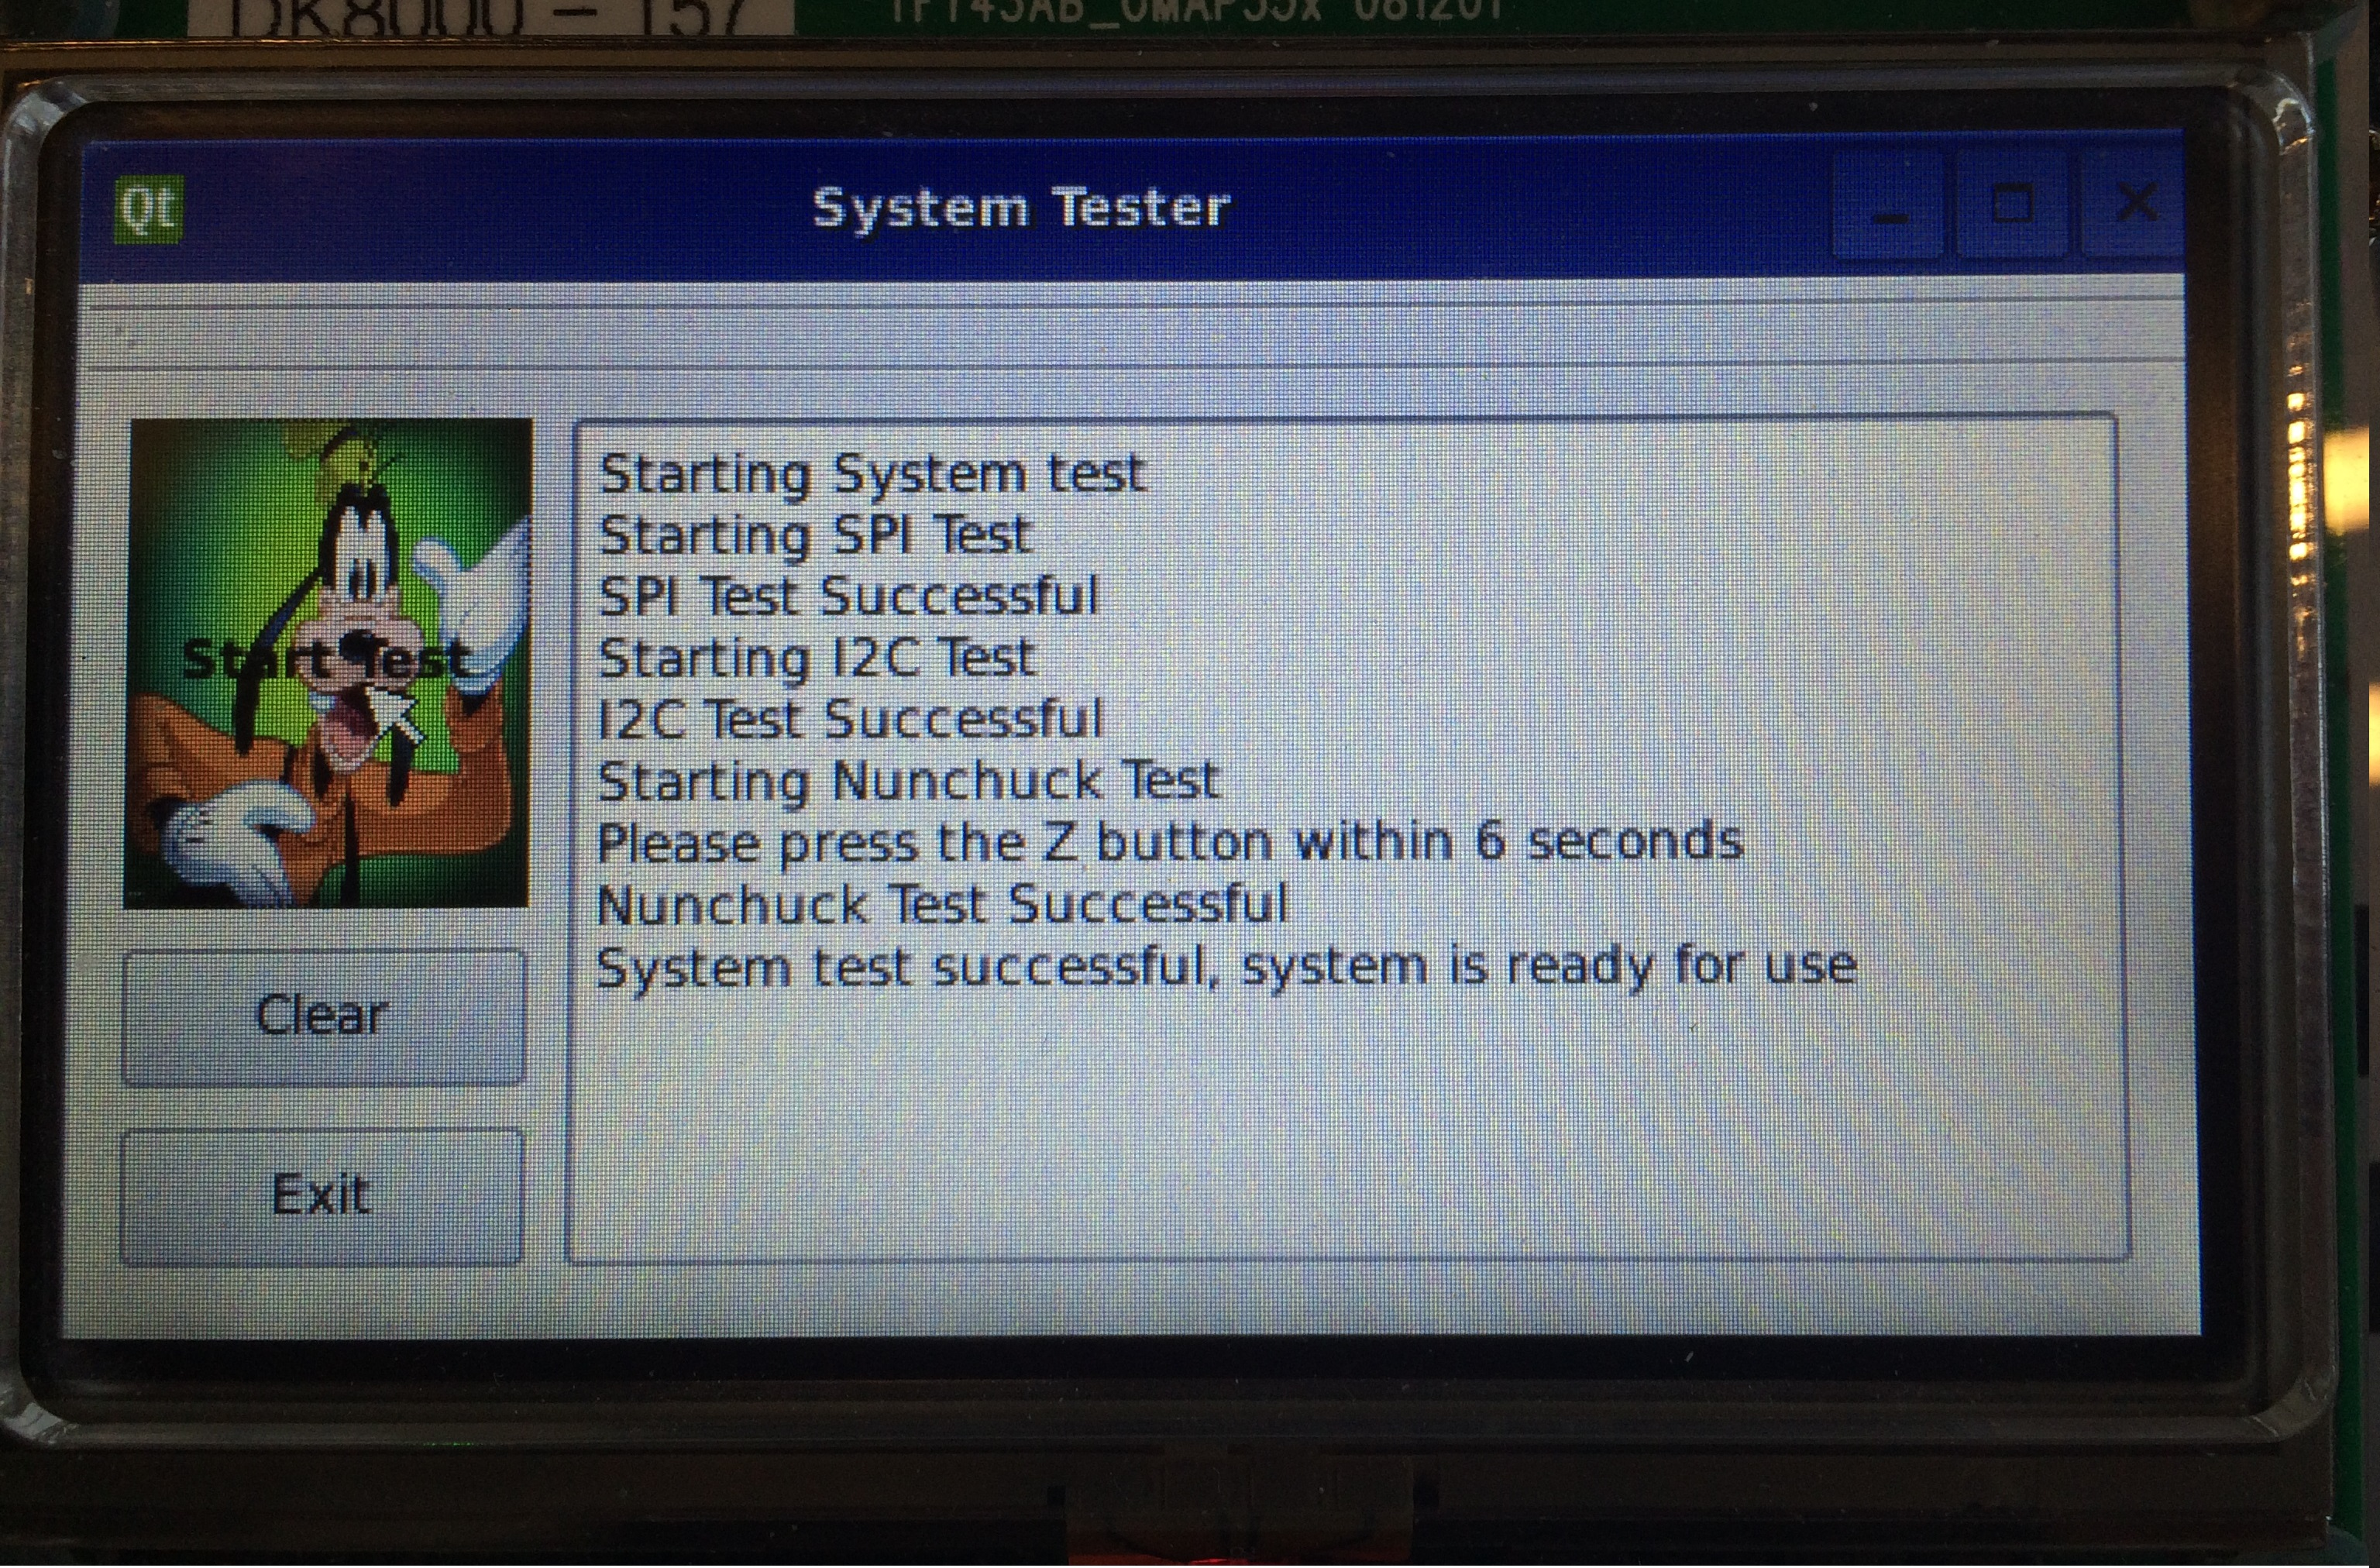
\includegraphics[width=\textwidth]{Test/images/IntegrationstestProtokoller/resultat2}
	\caption{Resultat af integrationstesten}
	\label{figure:integrationstestresult}
\end{figure}

Som det ses, er resultatet af testen som forventet, og testen er gennemført. Under testen bliver brugeren bedt om at trykke på nunchucken's 'z' knap. Hvis brugeren ikke klikker på knappen indenfor det angivne stykke tid, forventes det at testen vil fejle. Figur \ref{figure:integrationstestresult1} viser netop dette.


\begin{figure}[H]
	\centering
	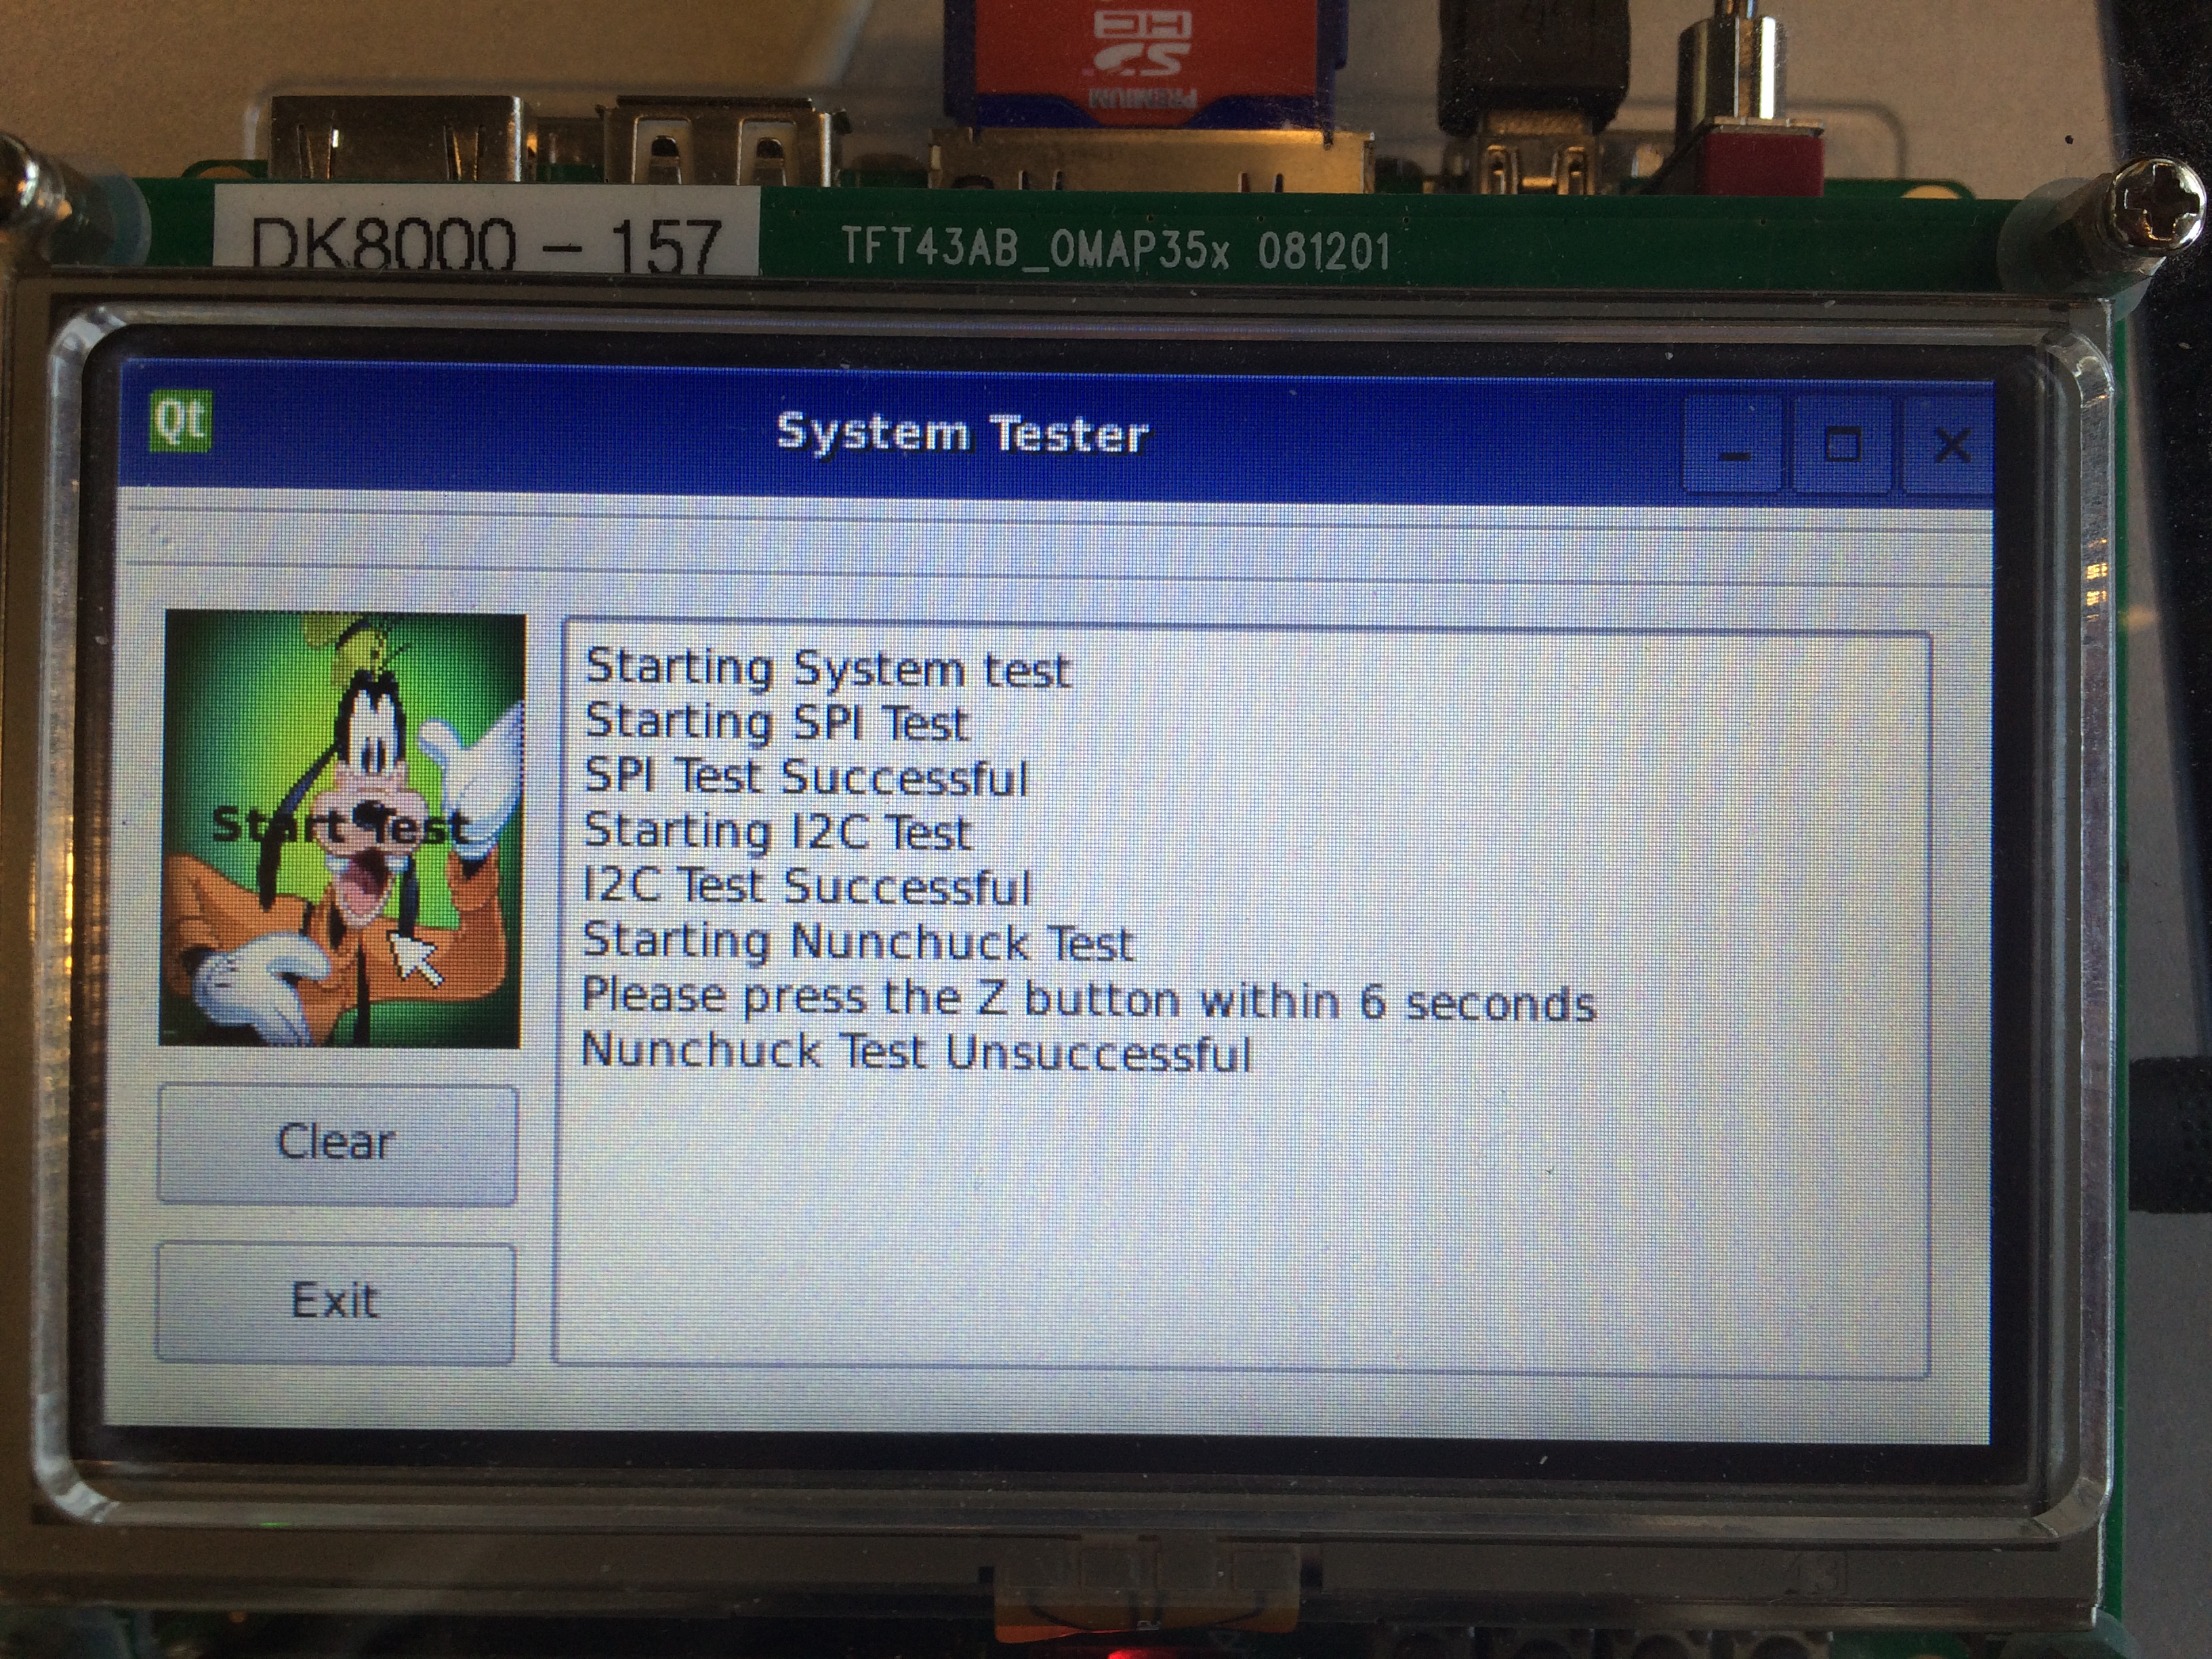
\includegraphics[width=\textwidth]{Test/images/IntegrationstestProtokoller/resultat1}
	\caption{Resultat hvis man ikke klikker på nunchuck}
	\label{figure:integrationstestresult1}
\end{figure}

Som det ses, fejlede testen, hvilket stemte overens med det forventede resultat. Derved kan det konkluderes at systemet opfører sig som forventet.

\section{Accepttest}